\documentclass[%
parskip=half-,%
fontsize=12pt,%
DIV=13,%
oneside,%
english,%
abstract=off,%
toc=chapterentrywithdots,toc=bibnumbered]{scrreprt}
\usepackage{fontspec}%	font specification, fuegt umlaute hinzu
\usepackage{libertine}%	font

\usepackage[svgnames*]{xcolor}%extended color, cmyk ist die Spezifizierung
\usepackage{color}

\setcounter{tocdepth}{4}%
\setcounter{secnumdepth}{4}%
\usepackage[backref=section]{hyperref}

\hypersetup{colorlinks=false}
\hypersetup{linkcolor=black}
\hypersetup{citecolor=teal}
\hypersetup{urlcolor=blue}
\hypersetup{linkbordercolor=orange}
\hypersetup{citebordercolor=orange}
\hypersetup{urlbordercolor=teal}
\hypersetup{linktoc=all}


\newcommand{\ts}{\textsuperscript}% allows to write 2\ts{nd} etc.
\newcommand\vsmallfont{\fontsize{6}{7.2}\selectfont}
\newcommand\smallfont{\fontsize{8.5}{9.7}\selectfont}
\newcommand\txtfont{\fontsize{11.5}{13.7}\selectfont}

\usepackage{listings}% to display SQL-code
\lstset{% settings for using listing-package
   basicstyle=\smallfont\ttfamily,% overall styl of text
   keywordstyle=\ttfamily\color{blue},% add \bfseries to display keyords (e.g., AS or CREATE) in bold
   stringstyle=\color{orange}\ttfamily,
   commentstyle=\color{gray}\ttfamily,
   emph=1,%{square}, 
   emphstyle=\color{blue}\texttt,
   emph=1,%{[2]root,base},
   %emphstyle={[2]\color{darkgreen}\texttt},
   showstringspaces=false,%do not show spaces in strings ("squat-u")
   flexiblecolumns=false,
   tabsize=2,
   numbers=left,
   numberstyle=\tiny,% fontsize of running-counter numbers
   numberblanklines=TRUE,% numbering of empty rows 
   stepnumber=1,% start running-counter or rows with
   numbersep=10pt,% vertical distance between numbers
   xleftmargin=25pt% distance of numbers from left 
 }


% it is apparantly possible to define postgreSQL as a new language, because using SQL as language results in highlighting of just a few keywords that are implmented in postgreSQL
\lstdefinelanguage{postgreSQL}{%
	  language     = SQL,
	morekeywords={%
		replace,%
		with,%
		::,%
		text,%
		boolean,%
		name,%
		void,%
		sign,%
		abs%,
		count,%
		round,%
		if,%
		begin,%
		return,%
		new,%
		old,%
		returns,%
		null,%
		nulls,%
		security,%
		definer,%
		language,%
		function,%
		functions,%
		procedure,%
		schema,%
		tables,%
		after,%
		before,%
		for,%
		each,%
		row,%
	}%
}

\usepackage{footnotebackref}


%\hypersetup{hyperfootnotes=false}

\deffootnote[1em]{1em}{2em}{\textsuperscript{\thefootnotemark\ }}

\usepackage{natbib}
\usepackage{cite}
\bibliographystyle{apsr}%apsr

\usepackage[headsepline,footsepline%,plainfootsepline
]{scrpage2}%	Kopf und Fusszeilen 
\pagestyle{scrheadings}%	seitenstil 

\usepackage{scrdate}% for using \the\year in page headings
\usepackage{datetime}% for using \monthname in page headings

\lohead{PCDB}%	left of head
\automark[section]{chapter}% defines structure (KOMA-Script manual, page 240ff.)
\renewcommand*{\sectionmarkformat}{}% adjusts section headmark foramt so that only section-title, but no section number is displayed
\cohead{\headmark}% places (Section-)mark in center of page-head
\rohead{\monthname\ \the\year}

%\usepackage{calc}
%\ifoot{\rule{0pt}{\ht\strutbox+\dp\strutbox}Footer}
\lofoot{Humboldt-University of Berlin}
\cofoot{}

\renewcommand*{\pnumfont}{\footfont}%let pagemark have same font&style like footfont
\rofoot{\pagemark}
\setheadsepline{.4pt}
%\setfootsepline{.4pt}

\usepackage{marginnote}%	erlaubt einfuegen von Randbemerkungen
\usepackage{varioref}%	erlaubt das Referenzieren von Abbildungen und Tabellen mit 							\ref{} und \pageref{}



\usepackage{ragged2e}%	erlaubt Flatteratz mit Trennung
\usepackage{array}%	 	erlaubt es neue Spaltentypen zu definieren

\newcolumntype{L}[1]% 	P: Kuerzel; 1: Anzahl der Parameter
{ >{\hspace{0pt}\RaggedRight} p {#1} }%definiert Spaltentyp der ohne Einrueckung 								beginnt und rechts flattert
\newcolumntype{R}[1]% 	P: Kuerzel; 1: Anzahl der Parameter
{ >{\hspace{0pt}\RaggedLeft} p {#1} }%definiert Spaltentyp der ohne Einrueckung 								beginnt und rechts flattert

\newcolumntype{C}[1]% 	P: Kuerzel; 1: Anzahl der Parameter
{ >{\hspace{0pt}\RaggedLeft\RaggedRight} p {#1} }%definiert Spaltentyp der ohne Einrueckung 								beginnt und rechts flattert

\usepackage{tabularx}% 	extended tabular
\usepackage{subcaption}
\usepackage{threeparttable}
\usepackage{longtable}

\DeclareCaptionLabelFormat{Uppercaselabel}{\MakeUppercase{#1 #2}}%Uppercase caption label (e.g. TABLE 1)
%\captionsetup[table]{labelformat=Uppercaselabel, labelsep=newline}%no collon but newline as sepaeartor of label and title 

\usepackage{dcolumn}
\usepackage{booktabs}
\usepackage{rotating}

\usepackage{setspace} % allows to set stretch in environemnents (e.g., \setstretch{.650})

\usepackage{url}
\urlstyle{same}

\usepackage{layout}
\newcommand*{\SubTitleFont}{%
      \usekomafont{title}%{\encodingdefault}{\rmdefault}{b}{n}%
      \fontsize{40}{30}%
      \selectfont}


\hypersetup{pdftitle = {Access to the Political Configurations Database}}
\hypersetup{pdfauthor = {Hauke Licht}}

\title{\huge Political Configurations Database}
\subtitle{\SubTitleFont\textbf{Documentation}\footnote{Last update: \today}}
\author{
	%Tarik Abou-Chadi, Ph.D.\thanks{Humboldt-University of Berlin}%
	\and%
	%Matthias Orlowski, Ph.D.\thanks{Humboldt-University of Berlin}%	
	\and%	
	%Hauke Licht\thanks{\href{mailto:hauke.licht.1@hu-berlin.de}{Contact: hauke.licht.1@hu-berlin.de}}%
	%\and
	%{\ss}% {\ss} produzeirt sz
	%\thanks{Freie Universität Berlin%Free University Berlin
	%}%
	%\and
	%Third Author%
	%\thanks{Institution}%
}
\publishers{
	Chair of Comparative Politics\\ Humboldt University of Berlin
	%Ellen M. Immergut, Professor Ph.D.\thanks{Humboldt University of Berlin}
	%\and%
	%Tarik Abou-Chadi, Ph.D.\thanks{Humboldt University of Berlin}%
	%\and%
	%Matthias Orlowski, Ph.D.\thanks{Humboldt University of Berlin}%
}
%\subject	{DFG-Project}
\date{\monthname\ \the\year}

\begin{document}



\chapter{Introduction}\label{chap_introduction}
The Political Configuration Database, short PCDB, is a compliation of \ldots
\newpage
\newpage

\chapter{The PCDB in \texttt{\bf pgAdmin}}\label{chap_the_PCDB_in_pgAdmin}

The PCDB is mostly easily accessed using the database managment and adminstration software \texttt{pgAdmin}.
You need to install \texttt{pgAdmin} on your computer,\footnote{Refer to \url{https://www.pgadmin.org/download/}} and connect to the PCDB on the server of the Humboldt-University, which is hosted by the Computer and Media Service (CMS).

The next couple of sections will provide a hands-on guide on 
how to connect to the PCDB on the CMS server (see \ref{sec_connecting_to_the_PCDB}),
how to query data from the PCDB (see \ref{sec_query_from_the_PCDB}), and
how to keep data in the PCDB up-to-date (see \ref{sec_keeping_the_PCDB_updated})
using the tools provided by with \texttt{pgAdmin3}.\footnote{When the first Pages of this Documentation were written, \texttt{pgAdmin4} was not available.}


\newpage
	\section{Connecting to the PCDB}\label{sec_connecting_to_the_PCDB}

After opening \texttt{pgAdmin3}, click `Add Server...' in the `File' tab of the program's menu bar, or click the toolbar icon looking like a plug; see figure \ref{fig_pgadmin3_add_server}).

\begin{figure}[h!]
\centering
  \begin{subfigure}{.45\textwidth}
  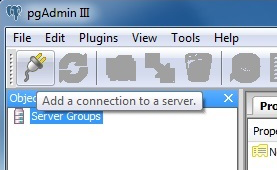
\includegraphics[width=\textwidth,trim= 0 0 0 0, clip]{pcdb_documentation_screenshots/pgadmin3_add_server.png}
    \subcaption{Click on plug icon to open `New Server Registration' interface.}
    \label{fig_pgadmin3_add_server}
  \end{subfigure}
  ~%
  \begin{subfigure}{.45\textwidth}
  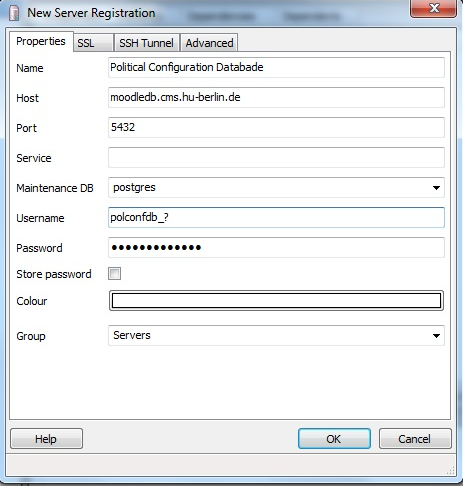
\includegraphics[width=\textwidth,trim= 0 0 0 0, clip]{pcdb_documentation_screenshots/pgadmin3_new_server_registration.png}
    \subcaption{Enter server information to `New Server Registration' interface.}
    \label{fig_pgadmin3_server_registration}
  \end{subfigure} 
  \caption{How to add and register a new server connection in \texttt{pgAdmin3}.}
\end{figure}

Enter the following properties of the PCDB in the corresponding lines of the Properties-tab of \texttt{pgAdmin3}'s `New Server Registration' wizard (see figure \ref{fig_pgadmin3_server_registration}):\\
\begin{itemize}
%Databasesysteme & \texttt{\footnotesize PostgreSQL} \\
\item[]{{\bf Name}: {\em Choose a name for the server connection!} (\texttt{\footnotesize Political Configuration Database} or \texttt{\footnotesize CMS Database} recomended)}
\item[]{{\bf Host}: \texttt{\footnotesize moodledb.cms.hu-berlin.de} }
\item[]{{\bf Port}: \texttt{\footnotesize 5432} }
%\item[]{{\bf SSL-Port}: \texttt{\footnotesize 5432} }
\item[]{{\bf Maintenance DB}: \texttt{\footnotesize postgres} }
\item[]{{\bf Username \& Password}: Contact \href{mailto:tarik.abou-chadi@hu-berlin.de}{the administrator} to receive a username and a user password! }
\end{itemize}
Please always unselect the `Store password' checkbox for security reasons! Finally, click `OK' to connect to the server.

\paragraph{In case you fail}
In case \texttt{pgAdmin3} prompts an error message on your server connection attempt in the `New Server Registration' wizar, read through carefully the error message and alos double-check your input (its likely that the error is due to a spelling error in your input). 
Always do some online research first (e.g., search the error message in Google or browse \texttt{pgAdmin3}'s documentation under \url{https://www.pgadmin.org/docs/dev/index.html}) in order to fix your problems. 

Should you not be able to fix your problem, and hence unablt to connect to the CMS database server, you can contact the CMS database service via email: \href{mailto:dbtech@cms.hu-berlin.de}{dbtech@cms.hu-berlin.de}
In case it turns out to be an issue with your version of \texttt{pgAdmin3}, contact your IT team (in the ISW this is Andreas Goroncy, \href{mailto:andreas.goroncy@sowi.hu-berlin.de}{andreas.goroncy@sowi.hu-berlin.de} or phone (030)~2093~4389).


\paragraph{In case you succeed}
Once you have successfully connected to the CMS database server, an element with the name you gave your server connection in the registration will appear in the `Object browser' (left panel below toolbar in \texttt{pgAdmin3}).  
Double-click on this icon to access the server. 

\begin{figure}[ht!]
\centering
  \begin{subfigure}{.45\textwidth}
  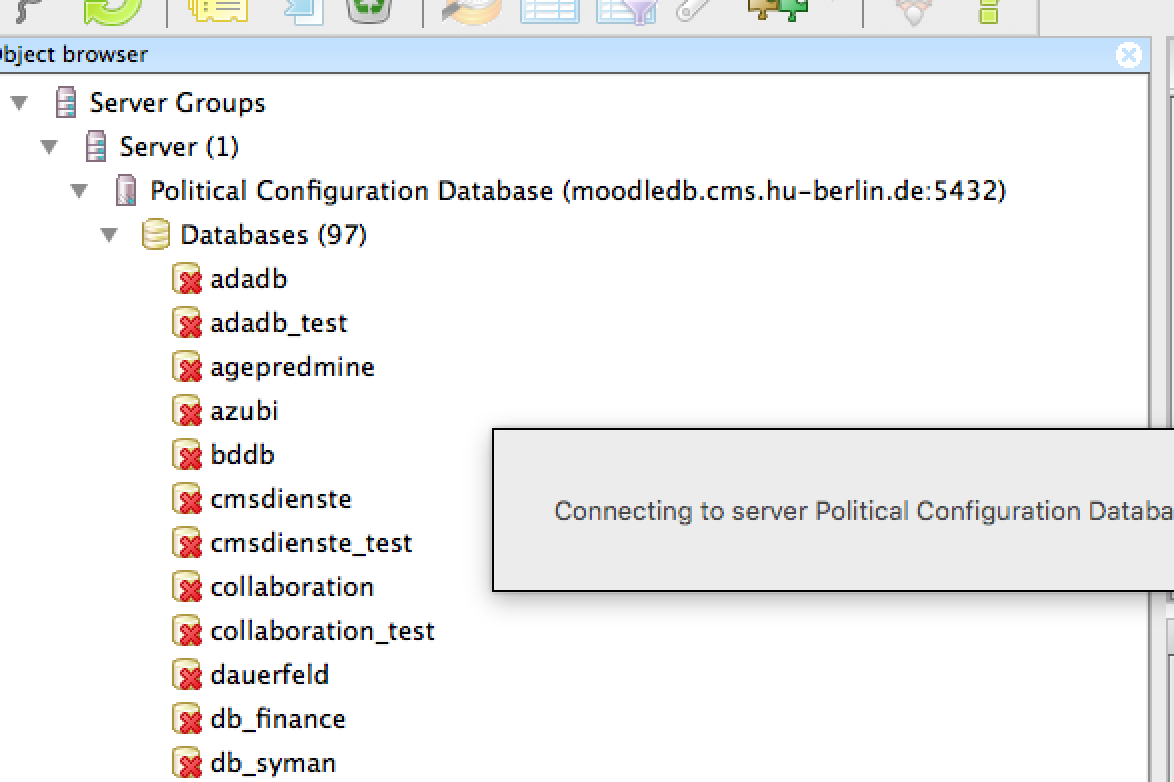
\includegraphics[width=\textwidth,trim= 0 0 0 0, clip]{pcdb_documentation_screenshots/pgadmin3_databases_on_server.png}
    \subcaption{View of `Object browser' window after connecting to the CMS database server.}
    \label{fig_pgadmin3_databases_on_server}
  \end{subfigure}
  ~%
  \begin{subfigure}{.45\textwidth}
  \includegraphics[width=\textwidth,trim= 0 0 0 0, clip]{pcdb_documentation_screenshots/pgadmin3_inside_pcdb.png}
    \subcaption{Inside the \texttt{polconfdb} database (PCDB) in the `Object browser' window.}
    \label{fig_pgadmin3_inside_pcdb}
  \end{subfigure} 
  \caption{Connecting to the CMS database server and accessing the PCDB in \texttt{pgAdmin3}.}
\end{figure}

Several databases will be associated in the `Object browser' with your server connection (see figure \ref{fig_pgadmin3_databases_on_server}).
The only database that is open to your access though is named \texttt{\footnotesize polconfdb} (see figure \ref{fig_pgadmin3_inside_pcdb}). (In contrast to the other databases, its icon is not visually marked with a red cross.) 

By default, to the right of the `Object browser' panel, you should see an information panel (upper-right, see figure \ref{fig_pgadmin3_inside_pcdb_information_panel}), and a `SQL pane' (lower-right panel, see figure \ref{fig_pgadmin3_inside_pcdb_SQL_pane}). 
The information panel always informs you about the properties, statistics, etc. of the object you have currently selected in the `Object browser,' and the `SQL pane' displays the definition of this object in SQL.

\begin{figure}[ht!]
\centering
  \begin{subfigure}{.45\textwidth}
  \includegraphics[width=\textwidth,trim= 0 0 0 0, clip]{pcdb_documentation_screenshots/pgadmin3_inside_pcdb_information_panel.png}
    \subcaption{View of `Object browser' window after connecting to the CMS database server.}
    \label{fig_pgadmin3_inside_pcdb_information_panel}
  \end{subfigure}
  ~%
  \begin{subfigure}{.45\textwidth}
  \includegraphics[width=\textwidth,trim= 0 0 0 0, clip]{pcdb_documentation_screenshots/pgadmin3_inside_pcdb_SQL_pane.png}
    \subcaption{`SQL pane' display for \texttt{polconfdb} database (PCDB).}
    \label{fig_pgadmin3_inside_pcdb_SQL_pane}
  \end{subfigure} 
  \caption{Information and SQL panels of the \texttt{polconfdb} database in \texttt{pgAdmin3}.}
\end{figure}

 	\newpage
	\section{Querying data from the PCDB}\label{sec_query_from_the_PCDB}

As figure \ref{fig_pgadmin3_inside_PCDB} shows, there are multiple schemas inside the PCDB. (Read about schemas in the \texttt{PostgreSQL} documentatin, \url{https://www.postgresql.org/docs/9.1/static/ddl-schemas.html})
The organization of the schemas in the PCDB is desribed in chapter \ref{chap_programming_the_PCDB}.

To browse a schema, simply select it with a doubl-click in the `Object browser.'
Selection by double-click will drop-down the objects inside the given schema, as shown in figure \ref{fig_pgadmin3_inside_config_data} for the \texttt{config\_data} schema inside the PCDB.

\begin{figure}[ht!]
\centering
  \begin{subfigure}{.45\textwidth}
  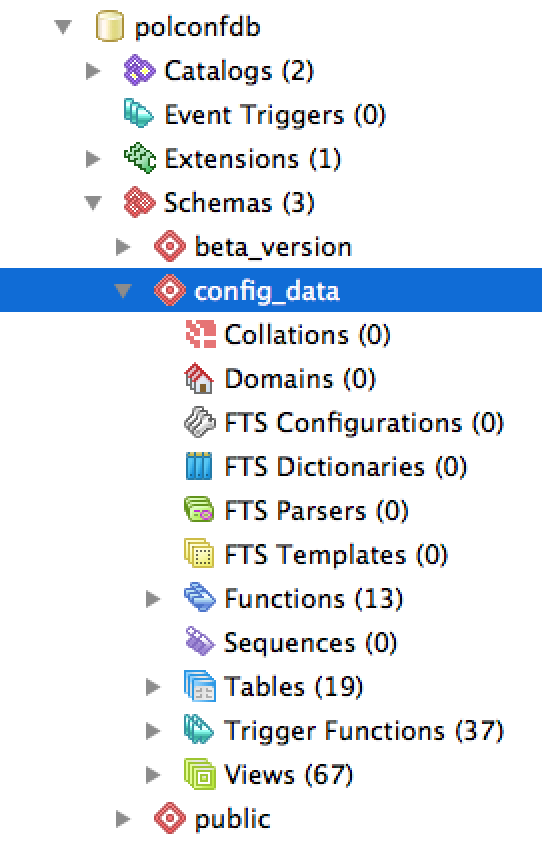
\includegraphics[width=\textwidth,trim= 0 0 0 0, clip]{pcdb_documentation_screenshots/pgadmin3_inside_config_data.png}
    \subcaption{View of `Object browser' window after selecting the \texttt{config\_data} schema of the \texttt{polconfdb} database in \texttt{pgAdmin3}.}
    \label{fig_pgadmin3_inside_config_data}
  \end{subfigure}
  ~%
  \begin{subfigure}{.45\textwidth}
  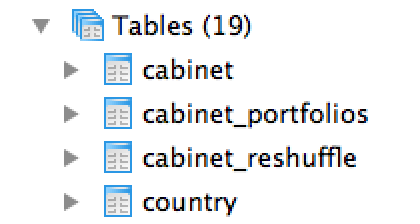
\includegraphics[width=\textwidth,trim= 0 0 0 0, clip]{pcdb_documentation_screenshots/pgadmin3_tables_inside_config_data.png}
    \subcaption{View of `Object browser' window after selecting tables in the \texttt{config\_data} schema of the \texttt{polconfdb} database in \texttt{pgAdmin3}.}
    \label{fig_pgadmin3_tables_inside_config_data}
  \end{subfigure} 
  \caption{Inside the \texttt{config\_data} schema of the \texttt{polconfdb} database in \texttt{pgAdmin3}.}
\end{figure}

There are a some contents you will usually be less concerned with, such as `Collations,' `Domains,' `FTS' objects, and `Sequences.' (Note that they are empty, as indicated by the zero in brackets after their names.)
Most important to you, in case you want to query data from the PCDB, are the `Tables' and `Views' objects.\footnote{
Tables are the permanent repositories that store the data of the PCDB; views are virtual tables based on the result-sets of pre-defined SQL-queries (queries are always executed when you query a view). Detailed descriptions of the content and definition of the tables and view in the PCDB are provided in chapter \ref{chap_programming_the_PCDB}.}
When you double-click on the `Tables' object in \texttt{pgAdmin3}'s `Object browser', a list of all tables in the current schema (here \texttt{config\_data}) will be displayed (see figure \ref{fig_pgadmin3_tables_inside_config_data}).

Double-clicking again on a particular table object will cause some changes in the tool bar: When selecting a particular table, the `Data Viewer' tool is activated (the icon that looks like a data table; right to the `SQL'-labeled magnifying glass, which is \texttt{pgAdmin3}'s built-in SQL-query editor).
The visual difference is shown in figures \ref{fig_pgadmin3_select_tables_toolbar} and \ref{fig_pgadmin3_select_a_table_toolbar}: 
When no particular table or view is selected, the `Data Viewer' icon is blured and not click-able (see figure \ref{fig_pgadmin3_select_tables_toolbar}); after selecting a particular table or view, you can double-click on the data viewer tool, and a data table window will pop up on your desktop.

\begin{figure}[ht!]
\centering
  \begin{subfigure}{.45\textwidth}
  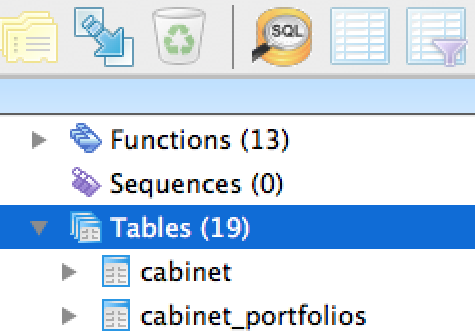
\includegraphics[width=\textwidth,trim= 0 0 0 0, clip]{pcdb_documentation_screenshots/pgadmin3_select_tables_toolbar.png}
    \subcaption{Tool bar when selecting `Tables' object in `Object browser' window.}
    \label{fig_pgadmin3_select_tables_toolbar}
  \end{subfigure}
  ~%
  \begin{subfigure}{.45\textwidth}
  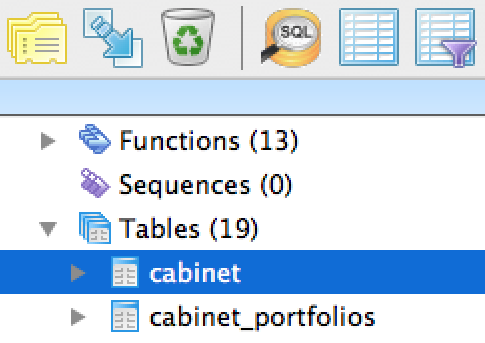
\includegraphics[width=\textwidth,trim= 0 0 0 0, clip]{pcdb_documentation_screenshots/pgadmin3_select_a_table_toolbar.png}
    \subcaption{Tool bar when selecting a particular table in `Object browser' window.}
    \label{fig_pgadmin3_select_a_table_toolbar}
  \end{subfigure} 
  \caption{Change in \texttt{pgAdmin3}'s tool bar when selecting a particular table.}
\end{figure}

  \subsection{Browse data in the PCDB: The `Data viewer' window}\label{subsec_data_viewer} 
Figure \ref{fig_pgadmin3_data_viewer_country} displayes the window that pops-up when selecting the country table in the \texttt{config\_data} schema in of the \texttt{polconfdb} database on the CMS database server.

\begin{figure}[ht!]
\centering
  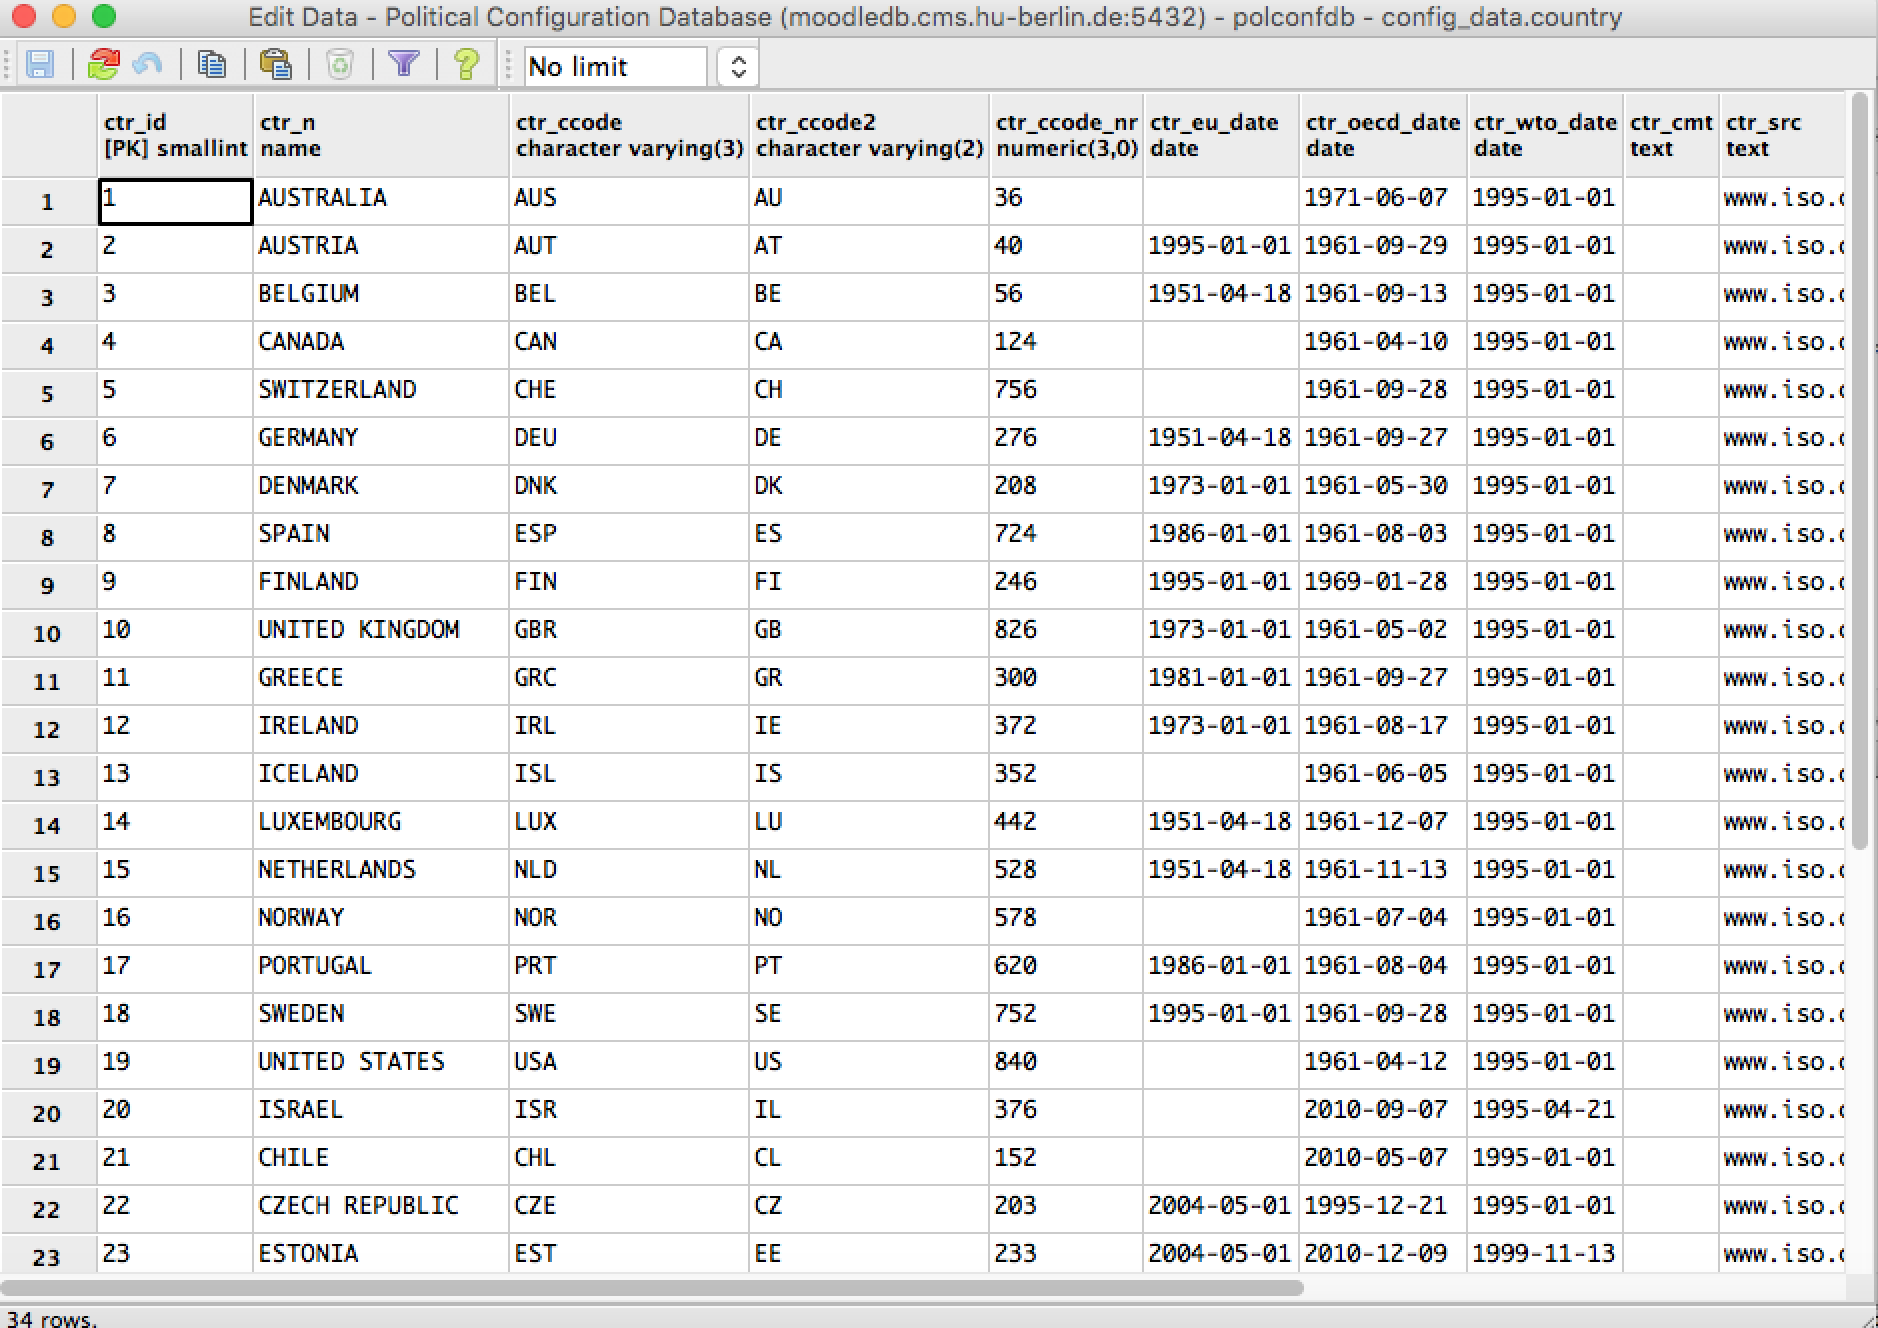
\includegraphics[width=.8\textwidth,trim= 0 0 0 0, clip]{pcdb_documentation_screenshots/pgadmin3_data_viewer_country.png}
    \caption{Data Viewer pop-up window of country table in \texttt{config\_data} schema.}
    \label{fig_pgadmin3_data_viewer_country}
\end{figure}

The `Data viewer' window has the following elements (from top to bottom):
\begin{itemize}
\item[-] The {\bf window header} informs you that this is an editor (i.e., if writing-rights are granted to your role, you can edit the data by double-clicking inside cells and change their content), and about the name of the server you are connected to (here ``Political Configuration Database''), the host and port number (``(moodledb.cms.hu-berlin.de:5432)''), as well as the database (``polconfdb''), and schema and table names (``config\_data.country''). This is in fact the all information you need to know which data table is displayed.

\item[-] The window's {\bf tool bar} allows you to refresh the current data table (icon with one red and one green circular arrow); and, in case you have writing rights, to save changes (blue shaded disc icon), or undo changes to the data (right-to-left upward-bend blue shaded arrow). 

\item[-] The {\bf main panel} displays the data of the selected table or view. 
Columns are variables, where the main panel's header displays variable names and types (e.g., \texttt{ctr\_id} and \texttt{smallint}), and contraints are displayed in square brackets (e.g., \texttt{[PK]}, which stands for primary key).
By default, all rows are listed; but you can limit the number of rows displayed in the most-right tool bar panel by typing a number in the input window label `No limit' by default.) 

\item[-] The {\bf window footer} informs you how many rows the displayed data has.
\end{itemize}

  \subsection{Export data from the PCDB: The SQL-query tool}\label{subsec_sql_query_tool}
While the `Data Viewer' only allows to view data (and to edit data only manually, one-by-one, in case you have writing-rights), \texttt{pgAdmin3}'s SQL-query tool allows to actually write and execute SQL-queries to obtain data from tables and views. 
Moreover, the SQL-Query tool allows to export the result-set of your query (a data table) to a file. 
Using the SQL-query tool is therefore the easiest way to export data from the PCDB.

Figure \ref{fig_pgadmin3_sql_query_tool_editor_country} and \ref{fig_pgadmin3_sql_query_tool_builder_country} show the two ways in which you may query data using the SQL-query tool, again using the example of of the country table in the \texttt{config\_data} schema.
\begin{itemize}
\item[(a)]{You may explicitly write SQL code to define a query in the `SQL Editor' tab of the SQL-query tool window's top panel. Double-clicking the green play-button in the SQL-query tool's toolbar (second from left in figure \ref{fig_pgadmin3_sql_query_tool_toolbar}) will execute the query; the result will be displayed as data table in the `Output pane' (bottom panel of the window).}
\item[(b)]{You may construct your query manually, using the in the `Graphical Query Builder' tab of the SQL-query tool window's top panel. Double-clicking the green play-button in the SQL-query tool's toolbar (second from left in figure \ref{fig_pgadmin3_sql_query_tool_toolbar}) will return the manually built query in explicit SQL code, execute it, and display the result as data table in the `Output pane' (bottom panel of the window).}
\end{itemize}

\begin{figure}[ht!]
\centering
  \begin{subfigure}{.45\textwidth}
  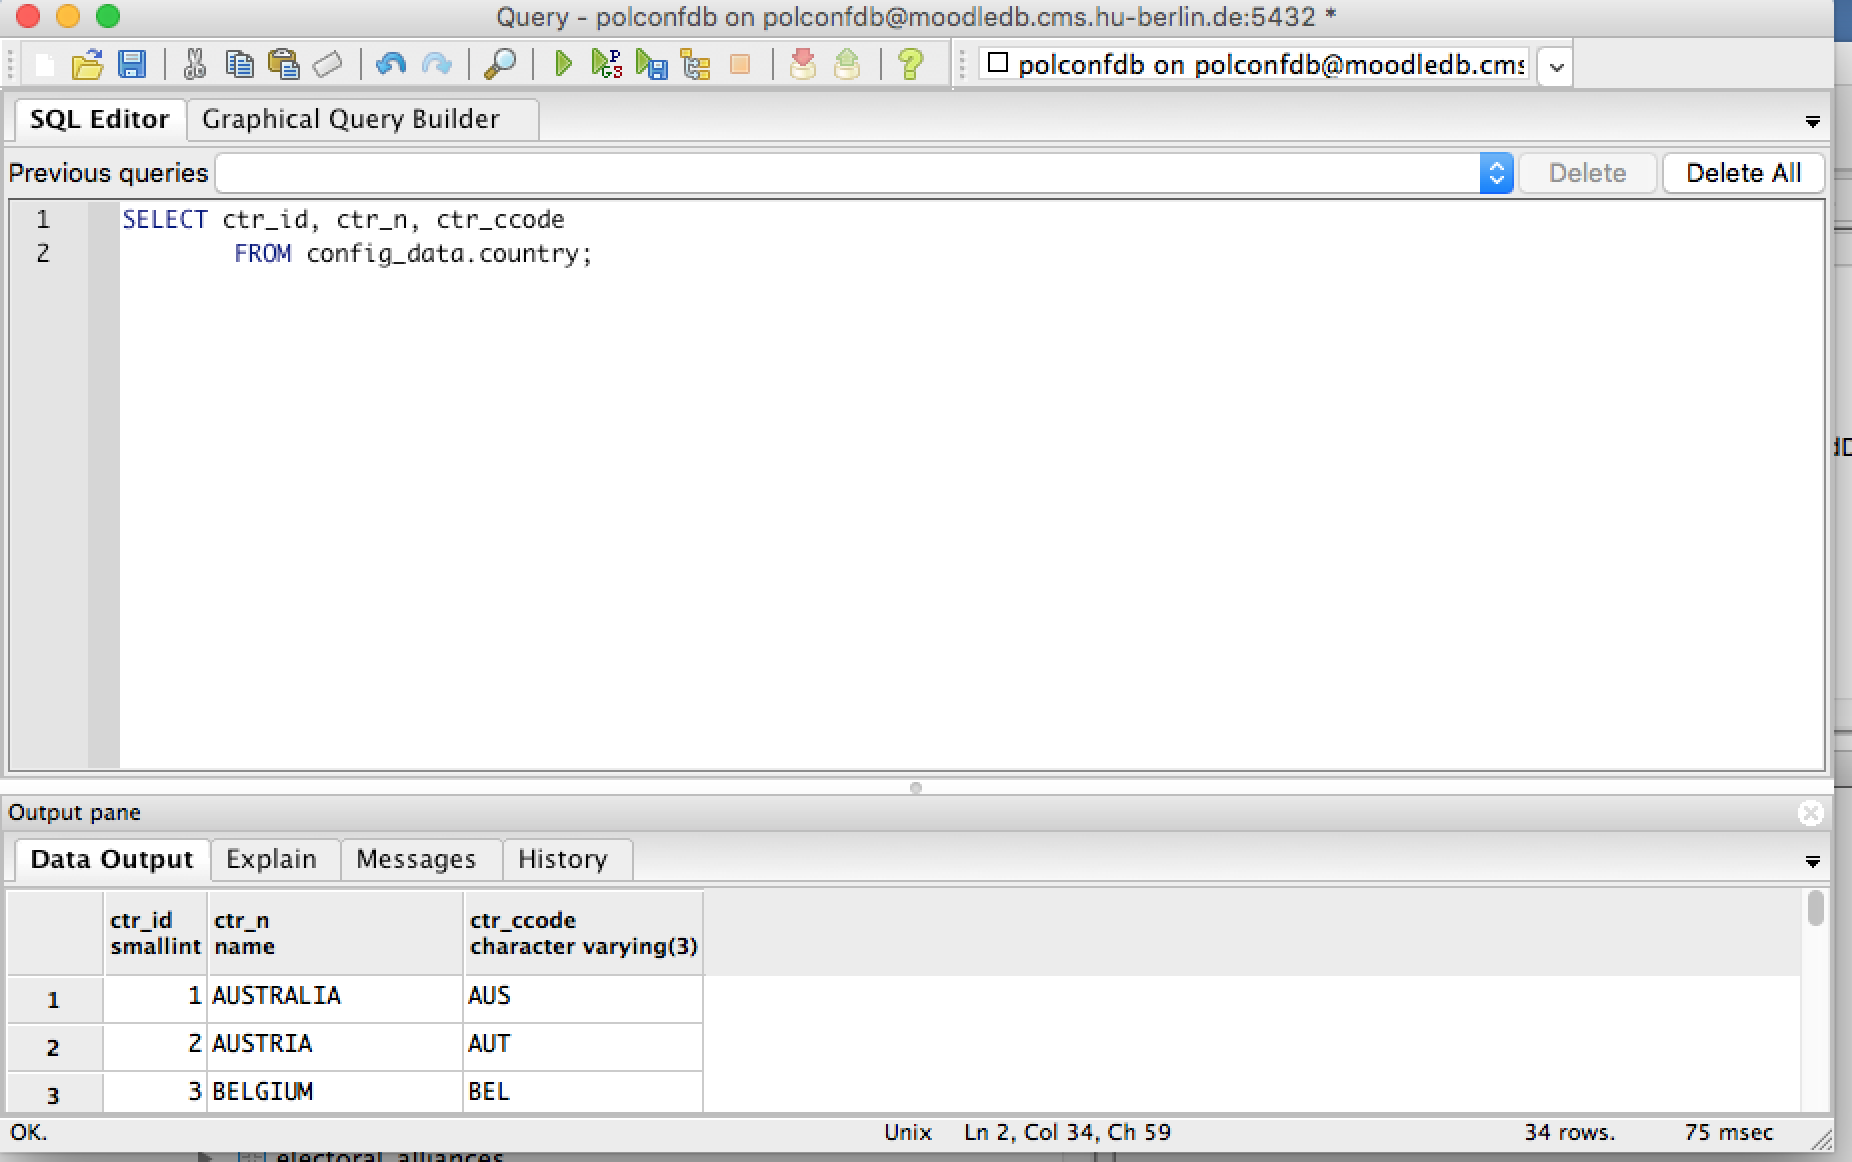
\includegraphics[width=\textwidth,trim= 0 0 0 0, clip]{pcdb_documentation_screenshots/pgadmin3_sql_query_tool_editor_country.png}
    \subcaption{Query data with explicit SQL code from country table in the `SQL Editor' tab.}
    \label{fig_pgadmin3_sql_query_tool_editor_country}
  \end{subfigure}
  ~%
  \begin{subfigure}{.45\textwidth}
  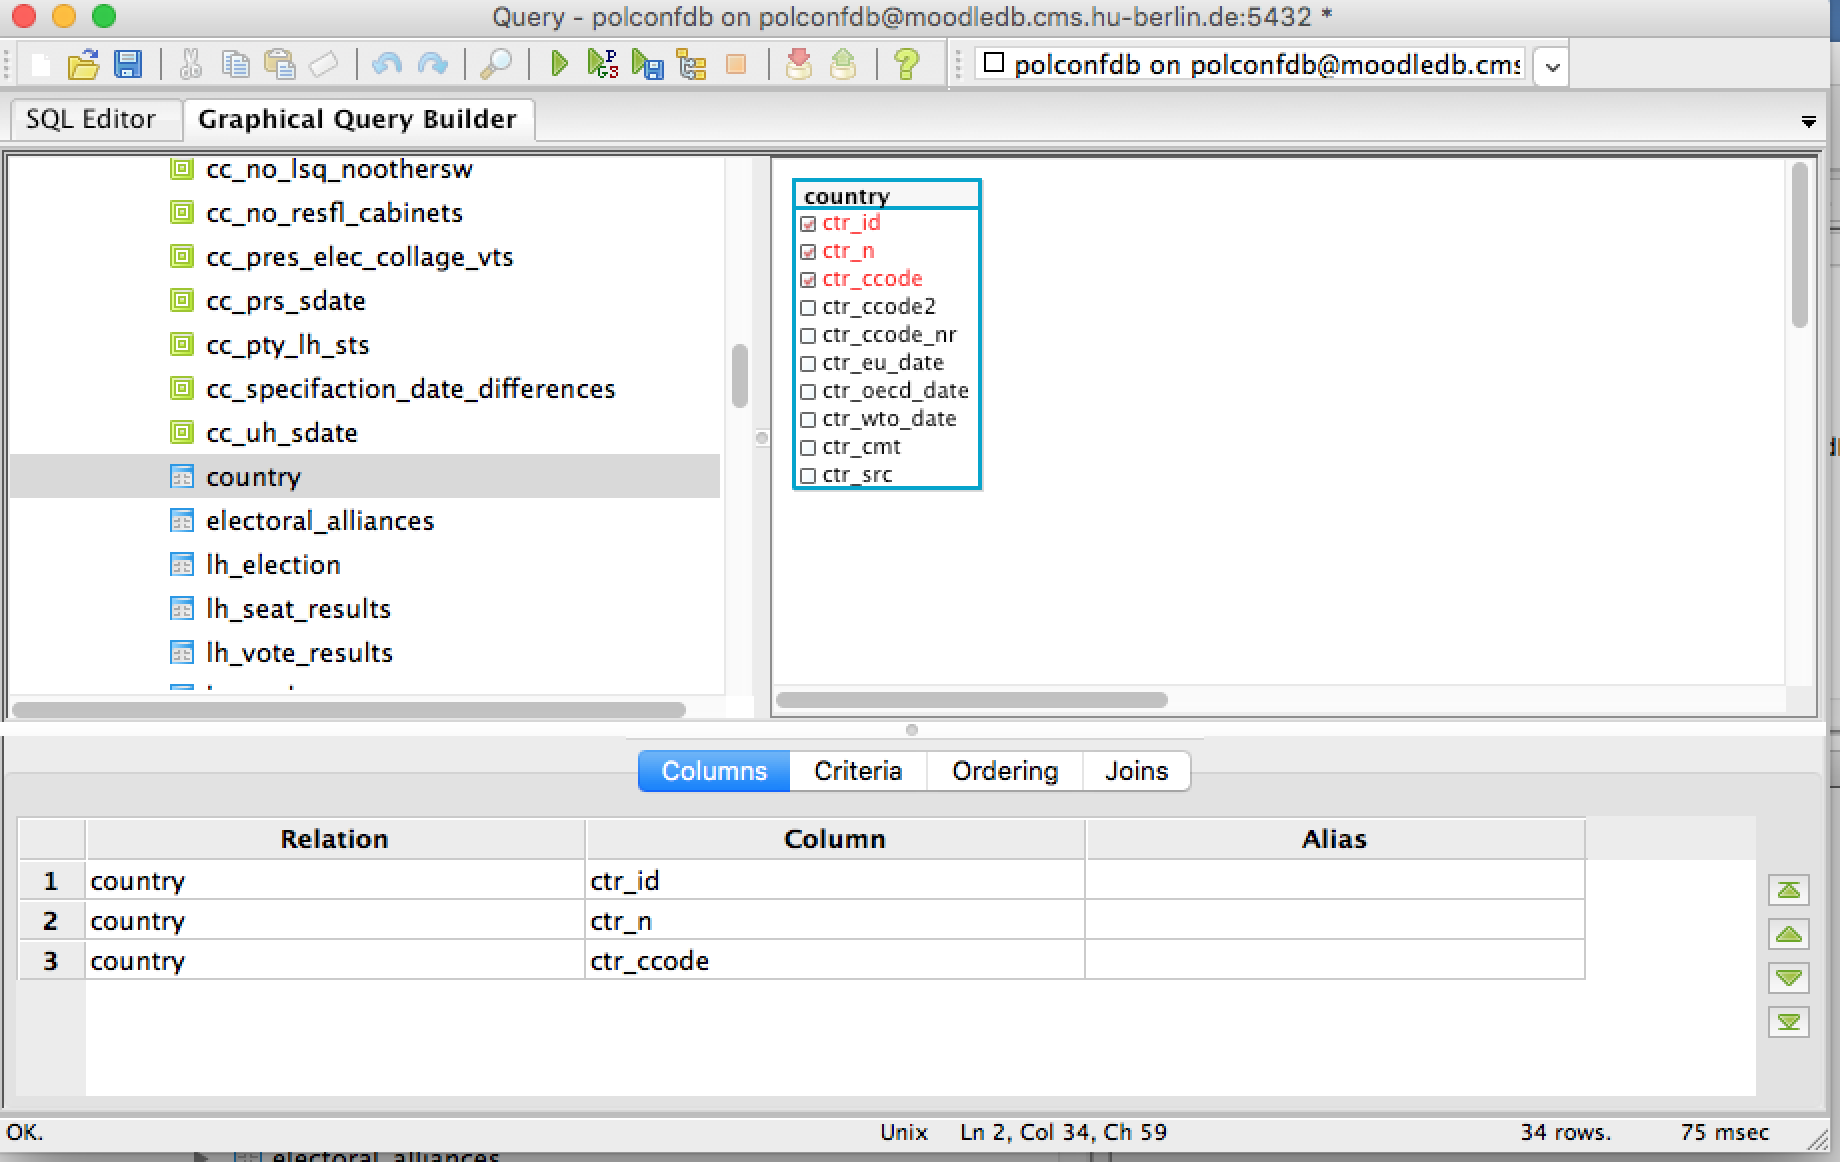
\includegraphics[width=\textwidth,trim= 0 0 0 0, clip]{pcdb_documentation_screenshots/pgadmin3_sql_query_tool_builder_country.png}
    \subcaption{Query data from country table  by manual selection in the `Graphical Query Builder' tab.}
    \label{fig_pgadmin3_sql_query_tool_builder_country}
  \end{subfigure} 
  \caption{Two ways to define queries in \texttt{pgadmin3}'s SQL-query tool window.}
\end{figure}

The double-clicking the green play-button in the SQL-query tool's toolbar (second from left in figure \ref{fig_pgadmin3_sql_query_tool_toolbar}) will execute the query; the result will be displayed as data table in the bottom panof the window.
The square shaped icon is the stop button (most right in figure \ref{fig_pgadmin3_sql_query_tool_toolbar}), which allows to cancel a running query.

\begin{figure}[ht!]
\centering
  
\includegraphics[width=.6\textwidth,trim= 0 0 0 0, clip]{pcdb_documentation_screenshots/pgadmin3_sql_query_tool_toolbar.png}
    \caption{Toolbar of \texttt{pgAdmin3}' SQL-query tool window.}
    \label{fig_pgadmin3_sql_query_tool_toolbar}
\end{figure}

The icon that combines a green play-button with a blue-shaded disc (third from right in figure \ref{fig_pgadmin3_sql_query_tool_toolbar}) will open the `Export data to file' wizard, which allows to write the result-set of a query to a file (see figure \ref{fig_pgadmin3_sql_query_tool_export_data_wizard}.
Select a column separator (default is a semicolon \texttt{;}), a quote character (default is the double qute \texttt{''}), select check-box `Column names' in case you want to include column (i.e., variable) names in the first row of the file, and select a path and file name to write to. Then click the `OK' button to export data to file.   

\begin{figure}[ht!]
\centering
  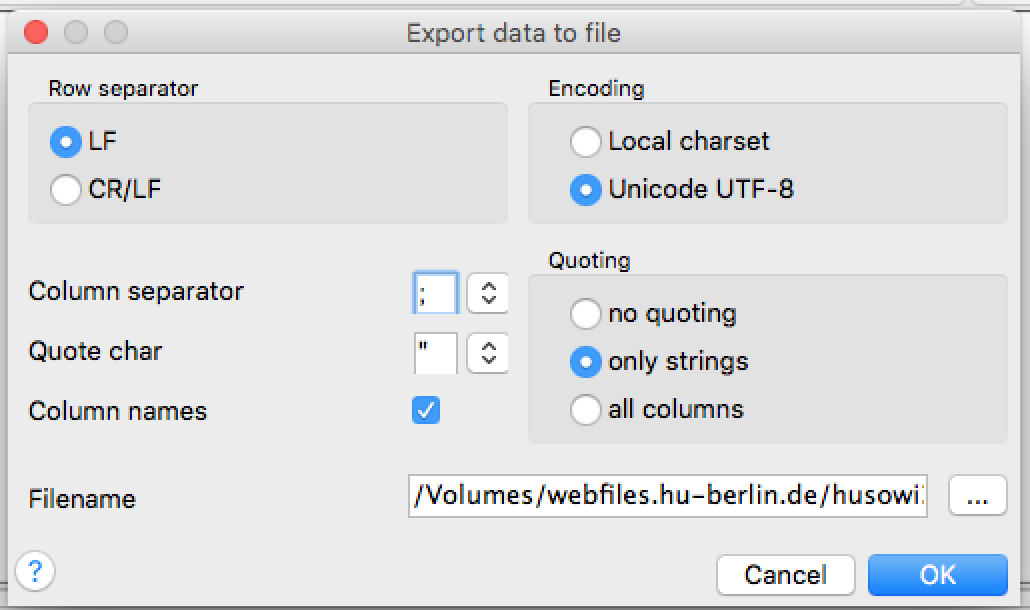
\includegraphics[width=.8\textwidth,trim= 0 0 0 0, clip]{pcdb_documentation_screenshots/pgadmin3_sql_query_tool_export_data_wizard.png}
    \caption{`Export data to file' wizard of \texttt{pgAdmin3}' SQL-query tool.}
    \label{fig_pgadmin3_sql_query_tool_export_data_wizard}
\end{figure}

When saving the result-set of the query to a file in the \texttt{.csv}-format, the result should look familiar to you. It's a plain semicolon-separated table (see figure \ref{fig_pgadmin3_sql_query_tool_export_data_result_example}).

\begin{figure}[ht!]
\centering
  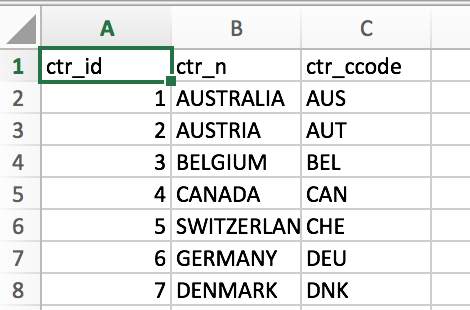
\includegraphics[width=.6\textwidth,trim= 0 0 0 0, clip]{pcdb_documentation_screenshots/pgadmin3_sql_query_tool_export_data_result_example.png}
    \caption{Result after exporting data with \texttt{pgAdmin3}'s `Export data to file' wizard.}
    \label{fig_pgadmin3_sql_query_tool_export_data_result_example}
\end{figure}





	\newpage
  \section{Keeping the PCDB updated}\label{sec_keeping_the_PCDB_updated}
I may also provide a guide how to insert, update, and delete data from the tables contained in the PCDB.
I have not yet developed any tool to insert data, e.g., from exel tables. Inserting a mass of data is thus far proceded manually, using SQL, and often painstacking.

%\lstinputlisting[%caption={Code to determine if the president constitutes an open veto point in a configuration.},
%language=SQL]%
%{../SQL-codes/view_configuration_vto_prs.sql}

The following paragraphs will use table Cabonet as an example to introdcue some minimal working examples (MWE) thought illustrate how data is inserted inot and deleted from the tables in the confgi\-data scheme, and how recorded date can be updated

THE MWEs can easily be transfered to the other base tables in the PCDB. 
However, it is imperative to stress that no data should be cahnged without having a clear idea of 
\begin{itemize}
\item[(a)]what is the primary key of a given table or the columns that uniquely identify rows;
\item[(b)]which referntial dependencies are implied by the structure of the PCDB; and accordingly,
\item[(c)]how incomplete insertation or updating, or thoughless deletion affects the integrity and constistency of the PCDB.
\end{itemize}

With respect to the MWE, 
(a) \texttt{\footnotesize cab\_id} is primary key of table Cabinet while additionally \texttt{\footnotesize cab\_sdate} in combination with \texttt{\footnotesize ctr\_id} uniquely identify observations, i.e., rows. 

With reespect to (b), \texttt{\footnotesize cab\_id} is referenced as foreign key in table Cabinet Portfolios and, in combination with \texttt{\footnotesize pty\_id}, uniquely identifies cabinet portfolios; table Cabinet being a base-table, \texttt{\footnotesize  cab\_id}s are sequenced in the Configuration view and thus are essential to compute configuration-specific indicators, such as veto constellations, and cabinet-parties seat share in the lower and upper houses; and \texttt{\footnotesize cab\_id}s are selected by several triggers to identify previous or subsequent cabinets for any given cabinet (subsections \ref{} and \ref{}).

Lastly, in view of (c), though it is possible to insert a new observation to table Cabinet without providing, for instance, its start date, this would cause non-trivial problems in compiling view Configurations and selecting it as next cabinet for the preceeding cabinet configuration, to name but few. Users are thus strongly inclined to pay attention to the key and uniquness characteristics of a given table when inserting, updating or deleting data from it-


\subsection{Insert}

Adding new row (i.e., an observation) to a table is proceeded with the \texttt{\footnotesize INSERT INTO}- command, specifying first the table, second the columns, and third the values to insert. Though insertation does not requiere to specify the destination-columns   when using the original order of columns of a table as default, specification is best-practice, as it guarantees for correctness of the procedure.
A MWE reads as follows:

\begin{lstlisting}[language=postgreSQL]
INSERT INTO config_data.cabinet
	(cab_id, ctr_id, cab_sdate, cab_hog_n, cab_care)
	VALUES (1036, 1, '2014-01-01', 'Abbott', 'FALSE');
\end{lstlisting}

Note that the values thought to insert need to match the specified types of the destination-columns. Typing instead 

\begin{lstlisting}[language=postgreSQL]
INSERT INTO config_data.cabinet
	(cab_id, ctr_id, cab_sdate, cab_hog_n, cab_care)
	VALUES (1036::NUMERIC(5,0), 1::SMALLINT, '2014-01-01'::DATE, 'Abbott'::NAME, 'FALSE'::BOOLEAN);
\end{lstlisting}

would thus avoid any surprises.

If one attempts to insert a value that does not match the type of the respective column, pgAdmin3 notes the error and states 
To recall the type of a given column, refer to the Codebook or browse the properties of the given table in  \texttt{\footnotesize pgAdmin3} (right click on table in menu bar, querying "")

It is generally recomended to refer to either the Codebook or Section X of the Manual, before inserting data into tables, as there are set constraints (e.g.,  \texttt{\footnotesize NOT NULL},  \texttt{\footnotesize PRIMARY KEY}, or  \texttt{\footnotesize UNIQUE}) on some of the columns that make insertation of a value obligatory when adding a new row to the table.

In addition, it is best-practice to assign ascending integer counters  to subsequent instituion configurations withn countries, thought the trigger structure that assigns identifiers of previous and next configurations to a current configuration does not require this order (see subsections \ref{trg_prv_ids} and \ref{trg_nxt_ids}).

Finally, remember that the primary key of the cabinet table, \texttt{\footnotesize cab\_id}, contributes to the unambigous identification of observations in the Cabinet Portfolio table. Following the tree of dependencies, inserting a new cabinet should be followed by specifying the correspoonding cabinet portfolio.
Also, information on the on the newly inserted cabinet's portfolio is requiered to obtained meaningful information on the political configuration (i.e., the lower house, upper house, and/or presidency cabient parties face) in which it is embedded.

\subsection{Update}

Altering the values of an existing row in a table is proceeded with the \texttt{\footnotesize UPDATE}-command, specifying the table and the column of the values that is thought to be updated. 
Updating is achieved by \texttt{\footnotesize SET}ting a column equal to some value that mathces the type of the respective column.
A \texttt{\footnotesize WHERE}-clause is requiered to identify the row(s) which are ment to be updated.
A MWE reads as follows:

\begin{lstlisting}[language=postgreSQL]
UPDATE config_data.cabinet 
	SET cab_sdate = '2014-03-15'::DATE 
	WHERE cab_id = 1036 
	AND ctr_id = 1 
	AND cab_sdate = '2014-01-01'::DATE;
\end{lstlisting}

Here, the value of the column that reports the cabinet's start date is updated in only one observation, as the attributes \texttt{\footnotesize cab\_id}, and \texttt{\footnotesize cab\_id} and \texttt{\footnotesize cab\_id}, respectively, uniquely identify rows in the Cabinet table.

It is possible to update information of more than one row.



  \newpage
  
\chapter{Data in the PCDB}\label{chap_data_in_the_PCDB}

This chapter provides a description of the data structre in the PCDB. 

Five entity types will be discussed:
\begin{itemize}
\item[]{{\bf Tables}: 
  The permanent data repositories that store information at different levels of aggregation (e.g., parties, institutions, countries, etc.) and serve as priamry source for all computed indices and aggregate figures.}
\item[]{{\bf Views}: 
  Virtual tables based on the result-sets of predefined SQL-queries.
  Views serve two purposes in the PCDB:
  \begin{itemize}
    \item[a)]Compute aggregates and indices from the primary data contained in tables,
    \item[b)]and create consistency checks that allow to control for the consistency of the data.
  \end{itemize}}
\item[]{{\bf Materialized views}: Tables created from views that may be updated from the original base tables as implemented by triggers and fucntions.}
\item[]{{\bf Triggers}: 
  Implemented on tables or materialized views to insert, update, or delete data as consequence of specific events. 
  Triggers are mainly implemented to enable the automatic up-dating of the data in the PCDB.}
\item[]{{\bf Functions}: The stored procedures to exectue predefined data manipulation operations when called.} 
\end{itemize}
 
\newpage
  \section{Roles in the PCDB}\label{sec_access_roles}

There exist three different roles with different sets of privileges to operate in the PCDB via \texttt{\footnotesize pgAdmin3}:
\begin{itemize}
\item[(1)]{{\bf Administrator}: Having all privileges on both the \texttt{\footnotesize public} and the \texttt{\footnotesize config\_data} schemes. 
This role is assumed by account \texttt{\footnotesize polconfdb} and \texttt{\footnotesize polconfdb\_1}. 
Having all privileges includes to \texttt{\footnotesize GRANT} and \texttt{\footnotesize REVOKE} privileges to and from other the user roles.}

\item[(2)]{{\bf Read-and-Write}: Having privileges  \texttt{\footnotesize SELCECT},  \texttt{\footnotesize INSERT}, and  \texttt{\footnotesize UPDATE} on both the \texttt{\footnotesize public} and the \texttt{\footnotesize config\_data} schemes. 
This role is assumed by account \texttt{\footnotesize polconfdb\_2} and \texttt{\footnotesize polconfdb\_3}.
Note that the  \texttt{\footnotesize SELECT}-privilege includes the operation  \texttt{\footnotesize COPY TO}, which allows to extract data from queries to  \texttt{\footnotesize .csv}-documents.}

\item[(3)]{{\bf Read-Only}: Having privilege \texttt{\footnotesize SELCECT} on both the \texttt{\footnotesize public} and the \texttt{\footnotesize config\_data} schemes. 
This role is assumed by account \texttt{\footnotesize polconfdb\_4} and \texttt{\footnotesize polconfdb\_5}.
The \texttt{\footnotesize SELECT}-privilege includes the operation  \texttt{\footnotesize COPY TO}.}
\end{itemize}

The roles in the PCDB are defined as follows:

\lstinputlisting[%caption={Code to compute the minimum-fragmentation Effective Number of Parties in Parliament.},%
language=postgreSQL]%
{../SQL-codes/define_roles.sql}
  \newpage
  \section{Tables in the \texttt{config\_data} schema}\label{sec_tables}

Tables store the primary data of the PCDB, that is used to compute aggregate figures and indices.
This section provides a description of how tables in the PCDB are defined, and thus provides a comprehensiv overview of variable names, their types (i.e., storage format), and potential constraints.

Both types and constraints define the requirements that data thought to be inserted into a column needs to met.\footnote{% 
An overview of the types provided within \texttt{PostgreSQL} can be found \href{http://www.postgresql.org/docs/9.3/static/datatype.html}{here}; information on constraints in tables \href{http://www.postgresql.org/docs/9.3/static/ddl-constraints.html}{here}.}

% In addition section the Appendix (see \ref{sec_appx_table_overview}) Appendix provides an overview of variables contained in the tables of the PCDB.
Figure \ref{fig_ER_diagram_PCDB} presents the entity-relationship model of the tables in the PCDB, including the focal cofiguration events and country-years materilaized views.

        
\newgeometry{left=1cm,right=1cm,bottom=1cm,top=0.5cm}
\begin{sidewaysfigure}
\centering
\begin{tikzpicture}[node distance=1cm]
\footnotesize
  %%%% CONFIGURATION LEVEL %%%%  
    
    \node (ConfEv) [table, text width=6cm, rectangle split, rectangle split parts=2]{
            \textbf{Configuration Events (Materialized) View}
            \nodepart{second}\underline{ctr\_id}, \underline{sdate},
                              cab\_id, lh\_id, lhelc\_id, uh\_id, prselc\_id,
                              \ldots
    };
    \node (ConfCtrYr) [table, text width=5cm, rectangle split, rectangle split parts=2, right=3cm of ConfEv]{
            \textbf{Configuration Country-Year (Materialized) View}
            \nodepart{second}\underline{ctr\_id}, \underline{year}, sdate, \ldots
    };
    
      %%% RELATIONSHIPS
      \draw[many_many_arrow] (ConfEv.east) -- (ConfCtrYr.west);

        
  %%%% BASE TABLE LEVEL %%%%

    \node (Upper House) [table, rectangle split, rectangle split parts=2, below=3cm of ConfEv] {
            \textbf{Upper House}
            \nodepart{second}\underline{uh\_id}, ctr\_id, uh\_sdate, \ldots
    };
    \node (Lower House) [table, rectangle split, rectangle split parts=2, left=of Upper House] {
            \textbf{Lower House}
            \nodepart{second}\underline{lh\_id}, ctr\_id, lh\_sdate, lhelc\_id, \ldots
    };
    \node (Cabinet) [table, rectangle split, rectangle split parts=2, left=of Lower House] {
            \textbf{Cabinet}
            \nodepart{second}\underline{cab\_id}, ctr\_id, cab\_sdate, \ldots
    };
    \node (Presidential Election) [table, rectangle split, rectangle split parts=2, right=of Upper House]{
            \textbf{Presidential Election}
            \nodepart{second}\underline{prselc\_id}, ctr\_id, prs\_sdate, \ldots
    };
    \node (Veto Points) [table, rectangle split, rectangle split parts=2, right=of Presidential Election]{
            \textbf{Veto Points}
            \nodepart{second}\underline{vto\_inst\_id}, ctr\_id, vto\_inst\_sdate, vto\_inst\_typ, \ldots
    };
    
    %%% RELATIONSHIP 
    \draw[many_one_arrow] (Upper House.north) -- ++(0,1.8) -| (ConfEv.south);
      \draw[line] (Upper House.north) -- ++(0,1.8) -| (Cabinet.north);
      \draw[line] (Upper House.north) -- ++(0,1.8) -| (Lower House.north);
      \draw[line] (Upper House.north) -- ++(0,1.8) -| (Presidential Election.north);
      \draw[line] (Upper House.north) -- ++(0,1.8) -| (Veto Points.north);
      
      %%% COMMENTS 
      \node[comment, above=.5cm of Upper House]{ctr\_id, uh\_sdate};
        \node[comment, above=.5cm of Cabinet]{ctr\_id, cab\_sdate};
        \node[comment, above=.5cm of Lower House]{ctr\_id, lh\_sdate};
        \node[comment, above=.5cm of Presidential Election]{ctr\_id, prs\_sdate};
        \node[comment, above=.5cm of Veto Points]{ctr\_id, vto\_inst\_sdate};
 
  %%%% PARTY LEVEL 
    \node (Party) [table, rectangle split, rectangle split parts=2, below=3.5cm of Veto Points]{
            \textbf{Party}
            \nodepart{second}\underline{pty\_id}, ctr\_id, pty\_abr, \ldots
    }; 
    \node (Cabinet Portfolios) [table, rectangle split, rectangle split parts=2, below=1.5cm of Cabinet]{
            \textbf{Cabinet Portfolios}
            \nodepart{second}\underline{ptf\_id}, cab\_id, pty\_id, \ldots
    }; 
      \draw[many_one_arrow] (Cabinet.south) -- (Cabinet Portfolios.north);
        \node[comment, above=.5cm of Cabinet Portfolios]{cab\_id};
    
%     \node (Minister) [table, rectangle split, rectangle split parts=2, below=3cm of Cabinet Portfolios]{
%             \textbf{Minister*}
%             \nodepart{second}\underline{min\_id}, cab\_id, cres\_id, pty\_id, min\_sdate, \ldots
%     }; 
%       \draw[many_one_arrow] (Cabinet.west) -- ++(-.5,0) |- ++(0,0) |-  (Minister.west);
%         \node[comment, above left=1cm and -.1cm of Minister]{cab\_id};
% 
%     \node (Cabinet Reshuffle) [table, rectangle split, rectangle split parts=2, below=1.5cm of Minister]{
%             \textbf{Cabinet Reshuffle*}
%             \nodepart{second}\underline{cres\_id}, cab\_id, cres\_cnt, cres\_date, pty\_id, \ldots
%     }; 
%       \draw[many_one_arrow] (Cabinet.west) -- ++(-.5,0) |- ++(0,0) |-  (Cabinet Reshuffle.west);
%         \node[comment, above left=.5cm and -.1cm of Cabinet Reshuffle]{cab\_id};


    \node (LH Seat Results) [table, rectangle split, rectangle split parts=2, below=1.5cm of Lower House]{
            \textbf{LH Seat Results}
            \nodepart{second}\underline{lhsres\_id}, lh\_id, pty\_id, \ldots
    }; 
       \draw[many_one_arrow] (Lower House.south) -- (LH Seat Results.north);
        \node[comment, above=.5cm of LH Seat Results]{lh\_id};

      \node (LH Vote Results) [table, rectangle split, rectangle split parts=2, below=3cm of LH Seat Results]{
              \textbf{LH Vote Results}
              \nodepart{second}\underline{lhvres\_id}, lh\_id, pty\_id, \ldots
      }; 
    \node (UH Seat Results) [table, rectangle split, rectangle split parts=2, below=1.5cm of Upper House]{
            \textbf{UH Seat Results}
            \nodepart{second}\underline{uhsres\_id}, uh\_id, pty\_id, \ldots
    }; 
      \draw[many_one_arrow] (Upper House.south) -- (UH Seat Results.north);
        \node[comment, above=.5cm of UH Seat Results]{uh\_id};
        
        
        \node (Presidential Election Vote Results) [table, rectangle split, rectangle split parts=2, below=1.5cm of Presidential Election]{
                \textbf{Presidential Election Vote Results}
                \nodepart{second}\underline{prsvres\_id}, prselc\_id, prselc\_rnd, prs\_cnd\_pty, \ldots
        }; 
          \draw[many_one_arrow] (Presidential Election.south) -- (Presidential Election Vote Results.north);
            \node[comment, above=.5cm of Presidential Election Vote Results]{prselc\_id};

      %%% RELATIONSHIPS
      \draw[many_one_arrow] (Party.west) -- ++(-2,0) -| (UH Seat Results.south);
      \draw[many_one_arrow] (Party.west) -- ++(-2,0) -| (LH Seat Results.south);
      \draw[many_one_arrow] (Party.west) -- ++(-2,0) -| (Presidential Election Vote Results.south);

      \draw[one_many_arrow] (Presidential Election.east) -- ++(.1,0) -| ++(.5,0) |- (Party.west);

      \draw[many_one_arrow] (Party.west) -- ++(-2,0) -| (LH Vote Results.north);

      % \draw[many_one_arrow] (Party.west) -- ++(-2,0) -| (Minister.north);
      % \draw[many_one_arrow] (Party.west) -- ++(-2,0) -| (Cabinet Portfolios.south);
        \node[comment, left=.1cm of Party]{pty\_id};
        \node[comment, left=2.5cm of Party]{pty\_id};
        \node[comment, left=7.75cm of Party]{pty\_id};
        \node[comment, left=13cm of Party]{pty\_id};
        \node[comment, left=18.25cm of Party]{pty\_id};

  %%%% ELECTION LEVEL %%%%
    \node (LH Election) [table, rectangle split, rectangle split parts=2, below=1.5cm of LH Vote Results]{
            \textbf{LH Election}
            \nodepart{second}\underline{lhelc\_id}, ctr\_id, lhelc\_date, \ldots
    }; 
       \draw[one_many_arrow] (LH Vote Results.south) -- (LH Election.north);
        \node[comment, above=.5cm of LH Election]{lhelc\_id};
       \draw[arrow] (LH Election.west) -- ++(-.5,0) |- ++(0,0) |- (Lower House.west);
        \node[comment, above left=.7cm and -.1cm of LH Election]{lhelc\_id};
        \node[zero_symbol, above left=.2cm and .37cm of LH Election]{};

    \node (UH Election) [table, rectangle split, rectangle split parts=2, below=6cm of UH Seat Results,]{
            \textbf{UH Election}
            \nodepart{second}\underline{uhelc\_id}, ctr\_id, uhelc\_date, \ldots
    }; 
       \draw[arrow] (UH Election.west) -- ++(-.5,0) |- ++(0,0) |- (Upper House.west);
        \node[comment, above left=.7cm and -.1cm of UH Election]{uhelc\_id};
        \node[zero_symbol, above left=.2cm and .37cm of UH Election]{};
  
  %%%% LEGEND %%%%
    \node (Legend) [legend, text width=5cm, rectangle split, rectangle split parts=2, below=2.2cm of Party]{
        \textbf{Legend}
        \nodepart{second} \vspace{2cm} 
    };
    %\node(one-to-one)[draw=none,fill=gray!10, below left=4.5cm and -2cm of Party ] {zero-or-one};
    \node(one-to-many)[legend_item, below left=3cm and -2cm of Party ] {one-to-many};
      \draw[many_one_arrow] (one-to-many) -- ++(3,0);
    \node(many-to-one)[legend_item, below left=3.5cm and -2cm of Party ] {many-to-one};
      \draw[one_many_arrow] (many-to-one) -- ++(3,0);
    \node(many-to-many)[legend_item, below left=4cm and -2cm of Party ] {many-to-many};
      \draw[many_many_arrow] (many-to-many) -- ++(3.15,0);
    \node(zero-or-one)[legend_item, below left=4.5cm and -2cm of Party ] {zero-or-one};
      \draw[arrow] (zero-or-one) -- ++(2.9,0); 
      \node[zero_symbol, right=.2cm of zero-or-one] {};

  \end{tikzpicture}
\medskip
\caption{Entity-relationship diagram of the tables in the \texttt{config\_data} schema of the PCDB.}
\end{sidewaysfigure}
\restoregeometry
\label{fig_ER_diagram_PCDB}

		\subsection{Country}\label{subsec_tab_country}
This table contains the 34 countries covered in the PCDB as rows, attributing each country a unique identifier (\texttt{\footnotesize ctr\_id}) and providing information on their accession date to specific international organizations. 

%The following countries (ISO3 country-code) are listed in the PCDB:
%\begin{table}[h!]
%\centering
%\caption*{List 1: ISO3 country-codes and names of countries recorded in the PCDB.}
%\input{../Codebook/tab_countries_in_PCDB}
%\end{table}

Table \texttt{\footnotesize country} is defined as follows:

\lstinputlisting[%caption={Code to compute the minimum-fragmentation Effective Number of Parties in Parliament.},%
language=postgreSQL]%
{../SQL-codes/tab_country.sql}

				
		\subsection{Party}\label{subsec_tab_party}
Table \texttt{\footnotesize party} provides basic information on parties, permitting to link them to other party-level databases or tables in the PCDB. 
Rows are parties within countries, identified by unique combinations of  \texttt{\footnotesize ctr\_id} and \texttt{\footnotesize pty\_id}.

\subparagraph{Party identifier}
The PCDB uses simple running counters to identify parties in a country's political system and history (variable \texttt{\footnotesize pty\_id}).
That is, in contrast to the coding schemes applied in the Manifesto Project \citep{ManifestoData2013} or the ParlGov data \citep{ParlGov2012}, identifiers do not encode allignment with party-families or ideological leaning on a left-right scale.

Special suffix are assigned to
independent candidates (\#\#997), 
other parties with seats (\#\#998), and 
other parties without seats in the legislature (\#\#999).
  
Table \texttt{\footnotesize party} is defined as follows: 

\lstinputlisting[%caption={Code to compute the minimum-fragmentation Effective Number of Parties in Parliament.},%
language=postgreSQL]%
{../SQL-codes/tab_party.sql}





		\subsection{Cabinets}\label{subsec_tab_cabinet}

Table \texttt{cabinet} contains information on cabinets.
Rows are the different cabinet configurations, identified by variable \texttt{cab\_id}. 
A new cabinet is enlisted if one of the following events took place:
\begin{itemize}\label{cabinet_change_criteria}\itemsep-4pt \parsep0pt
\item[a)] Coalition composition changes at the party-level.
\item[b)] Head of government changes.
\item[c)] Government formation after general legislative elections (not in presidential systems).
\end{itemize}

\subparagraph{Cabinet start date} Variable \texttt{cab\_sdate} refers to the date on which the cabinet, as proposed by the Head of Government, recieves a vote of confidence in the legislature. The variable \texttt{cab\_src} regularly contains links to the websites or online repositories which are used as references. If available, data was compiled directly from information reported on government websites or other official sources.

\subparagraph{Total number of cabinet portfolios} In the present version of the database (!) the number of cabinet portolios is an integer counter equal to the number of parties in cabinet. 
Because it is an aggregate of data contained in the Cabinet Portfolios table (\ref{subsec_tab_cabinet_portfolios}), the total number of cabinet portfolios is cumputed in \texttt{view\_pty\_cab\_sts} (\ref{view_pty_cab_sts}).

%\subparagraph{Sources} Information is obtained from \citet*{Woldendrop_et_al2000} and the Political Data Yearbook \citeyearpar{EJPR_PDY}, and was complemented by individual-case research.

\subparagraph{}
Table \texttt{cabinet} is defined as follows:
\lstinputlisting[%caption={Code to compute the minimum-fragmentation Effective Number of Parties in Parliament.},%
language=postgreSQL]%
{../SQL-codes/tables/tab_cabinet.sql}


		\subsection{Cabinet Portfolios}\label{subsec_tab_cabinet_portfolios}
Table \texttt{cabinet\_portfolios} provides information on parties in cabinets. 

As cabinet portfolio we define the composition of a cabinet at the party-level.
%, i.e., the parties that form the, government, the number of a party’s share on total cabinet seats, and parties supporting government. 
Thus, new portfolios are included whenever a new cabinet emerges.
The changes that occur at the party-level regularly correspond to the events enumerated as criteria for recording a new cabinet configuration (cf. subsection \ref{subsec_tab_cabinet}):
\begin{itemize}%\itemsep-4pt \parsep0pt
\item[a)] Coalition composition changes.
\item[b)] Head of government changes.
\item[c)] Government formation after general legislative elections (not in presidential systems).
\end{itemize}
Obviously, combinations of cabinet and party identifier are unique in the cabinet portfolios table.

Table \texttt{cabinet\_portfolios} is defined as follows:
\lstinputlisting[%caption={Code to compute the minimum-fragmentation Effective Number of Parties in Parliament.},%
language=postgreSQL]%
{../SQL-codes/tables/tab_cabinet_portfolios.sql}

		
		\subsection{Lower House}\label{subsec_tab_lower_house}
Table \texttt{\footnotesize lower\_house} provides information on lower houses.
Rows are compositions of lower houses, identified by \texttt{\footnotesize lh\_id}. 

A new lower house configuration is included when the seat composition is changed through legislative elections or through mergers or splits in factions during the legislature. When enlistment is due to the latter event, no lower house 
election identifier (\texttt{\footnotesize lhelc\_id}) is recorded. Else, each lower house corresponds to a lower house election.

\subparagraph{Lower house start date}
PCDB codes the date of the first meeting in the first legislative session of a new lower house as its start date (variable \texttt{\footnotesize lh\_sdate}). Information on the sources is provided in variable \texttt{\footnotesize lh\_src}. If no information on this event is available, the default is equal to the corresponding election date. 

\subparagraph{Total number of seats in lower house} 
The figures on the total number of seats in the respective lower house are recorded in accordance with official electoral statistics (variable \texttt{\footnotesize lh\_sts\_ttl}). These figures do not necessarily equal the sum of all seats distributed between different parties of a legislature (as recorded in the lower house seat reuslts data,  see subsection \ref{sub_tab_lh_seat_results}).

Table \texttt{\footnotesize lower\_house} is defined as follows:

\lstinputlisting[%caption={Code to compute the minimum-fragmentation Effective Number of Parties in Parliament.},%
language=postgreSQL]%
{../SQL-codes/tab_cabinet.sql}

		\subsection{Lower House Election}\label{subsec_tab_lh_election}
Table \texttt{\footnotesize lh\_election} provides information on lower house elections. 
Rows are lower house elections, identified by \texttt{\footnotesize lhelc\_id}. It is noteworthy that each lower house election corresponds to a lower house configuration (cf. subsection \ref{subsec_tab_lower_house}).\footnote{While the opposite, that each lower house configuration corresponds to a lower house election, is not true.}

\subparagraph{Elections, pluarality versus proportional voting, and seat allocation}
Lower house election dates (\texttt{\footnotesize lhelc\_date}), and figures on registered voters (\texttt{\footnotesize lhelc\_reg\_vts*}), the number valid votes (\texttt{\footnotesize lhelc\_vts\_*}), and the number of seats elected (\texttt{\footnotesize lhelc\_sts\_*}) are recorded in accordance with official statistics, if available. 
Else, \citet{Nohlen2001, Nohlen2005, Nohlen2010} is the primary source, complemented by individual-case research. Information on data sources is provided in variable \texttt{\footnotesize lhelc\_src}.

\subparagraph{Electoral system}
Key information on the electoral system to elect the lower house is provided for each tier disaggregatedly namely
\begin{itemize}\itemsep-4pt \parsep0pt
\item[-]{the electoral formular (\texttt{\footnotesize lhelc\_fml\_t*}), as defined by a customed type \texttt{\footnotesize elec\_formula}
%\footnote{The PCDB distinguishes between the following electural formular: Two Round System (2RS), Alternative Vote (AV), DHondt, Droop, Droop with Largest-Remainders (LR-Droop), Hare, modified Hare, Hare with Largest-Remainders (LR-Hare), Highest Average Remaining, Imperiali, Multi-Member District (MMD), mSainteLague, Reinforced Imperiali, SainteLague, Single Member Plurality (SMP), Single Non-Transferable Vote (SNTV), and Single Transferable Vote (STV).%}
,}
\item[-]{the number of constituencies (\texttt{\footnotesize lhelc\_ncst\_t*}),}
\item[-]{the number of seats allocated(\texttt{\footnotesize lhelc\_sts\_t*}),}
\item[-]{the average district magnitude (\texttt{\footnotesize lhelc\_mag\_t*}),}
\item[-]{the national threshold (\texttt{\footnotesize lhelc\_ntrsh\_t*}), and}
\item[-]{the district threshold (\texttt{\footnotesize lhelc\_dtrsh\_t*}).}
\end{itemize}
Type \texttt{\footnotesize elec\_formula} is defined as follows:
\lstinputlisting[%caption={Code to compute the minimum-fragmentation Effective Number of Parties in Parliament.},%
language=postgreSQL]%
{../SQL-codes/type_elec_formula.sql}

In addition, 
%\subparagraph{Mean and median average district magnitude}
variables \texttt{\footnotesize lhelc\_dstr\_mag} and \texttt{\footnotesize lhelc\_dstr\_mag\_med} aggregate the average district magnitudes across the different tiers of the electoral system, reporting the mean and the median, respectively.

Comments and information on the sources of data on the electoral system are provided in \texttt{\footnotesize lhelc\_esys\_cmt} and \texttt{\footnotesize lhelc\_esys\_src}, respectively.

Table \texttt{\footnotesize lh\_election}  is defined as follows:

\lstinputlisting[%caption={Code to compute the minimum-fragmentation Effective Number of Parties in Parliament.},%
language=postgreSQL]%
{../SQL-codes/tab_lh_election.sql}

		\subsection{Lower House Vote Results}\label{subsec_tab_lh_vote_results}
Table \texttt{\footnotesize lh\_vote\_results} contains data on the distribution of votes in the lower house at the party-level. 
Rows are the parties (identified by variable \texttt{\footnotesize pty\_id}) and their respective vote results in a given lower house election (variable \texttt{\footnotesize lh\_id}).

%Information is obtained  from \citeauthor{Nohlen2001} (\citeyear{Nohlen2001}, \citeyear{Nohlen2005}, \citeyear{Nohlen2010}), and complemented by individual-case research. Weblinks to or citation of individual sources are provided either in \texttt{\footnotesize lhvres\_src}, or the general source information on the correponding lower house election (\texttt{\footnotesize lhelc\_src} in Table \ref{tab_lh_election}).

It is defined as follows: 

\lstinputlisting[%caption={Code to compute the minimum-fragmentation Effective Number of Parties in Parliament.},%
language=postgreSQL]%
{../SQL-codes/tab_lh_vote_results.sql}


		\subsection{Lower House Seat Results}\label{subsec_tab_lh_seat_results}
Table \texttt{lh\_seat\_results} contains data on the distribution of seats in the lower house at the party-level. 
Rows are the parties (identified by variable \texttt{pty\_id}) and their respective vote results in a given lower house election (variable \texttt{lh\_id}).

%Information is obtained  from \citeauthor{Nohlen2001} (\citeyear{Nohlen2001}, \citeyear{Nohlen2005}, \citeyear{Nohlen2010}), and complemented by individual-case research. Weblinks to or citation of individual sources are provided either in \texttt{lhvres\_src}, or the general source information on the correponding lower house election (\texttt{lhelc\_src} in Table \ref{tab_lh_election}).

It is defined as follows: 
\lstinputlisting[%caption={Code to compute the minimum-fragmentation Effective Number of Parties in Parliament.},%
language=postgreSQL]%
{../SQL-codes/tables/tab_lh_seat_results.sql}


 	
		\subsection{Upper Houses}\label{subsec_tab_upper_house}
Table \texttt{upper\_house} provides basic information on upper houses, including start date of legislature and the total number of seats. 
Rows are compositions of upper houses, identified by \texttt{uh\_id} as well as unique combinations of \texttt{ctr\_id} and \texttt{uh\_sdate}.
 
A new upper house composition is included when
\begin{itemize}%\itemsep-4pt \parsep0pt
\item[a)]the composition changes through legislative elections, or
\item[b)]mergers or splits in factions occur during the legislature.
\end{itemize} 
Only countries with bicameral systems are recorded.

\subparagraph{Upper house start date}
PCDB codes the date of the first meeting in the first legislative session of a new upper house as its start date. 
If no information on these events was available, the default is equal to the corresponding election date. 
%The table contains the following variables:

\subparagraph{}
Table \texttt{upper\_house} is defined as follows:
\lstinputlisting[%caption={Code to compute the minimum-fragmentation Effective Number of Parties in Parliament.},%
language=postgreSQL]%
{../SQL-codes/tables/tab_upper_house.sql}


		\subsection{Upper House Elections}\label{subsec_tab_uh_election}

Table \texttt{uh\_election} includes information on upper house elections. 
Rows report elections to form the upper house, and are identified by \texttt{uhelc\_id} as well as unique combinations of \texttt{ctr\_id} and \texttt{uhelc\_date}. 
Information is only provided for countries with bicameral systems.

It is defined as follows:
\lstinputlisting[%caption={Code to compute the minimum-fragmentation Effective Number of Parties in Parliament.},%
language=postgreSQL]%
{../SQL-codes/tables/tab_uh_election.sql}

		\subsection{Upper House Seat Results}\label{subsec_tab_uh_seat_results}
Table  \texttt{\footnotesize uh\_seat\_results} compiles data on the seat composition in upper houses at the party-level. 
Rows are the parties, identified by variable \texttt{\footnotesize pty\_id}, and their respective seat results in a given upper house (\texttt{\footnotesize uh\_id}).

%Information is obtained from \citeauthor{Nohlen2001} (\citeyear{Nohlen2001}, \citeyear{Nohlen2005}, \citeyear{Nohlen2010}), and was complemented by individual-case research. Weblinks to, or citations of individual sources are provided either in \texttt{\footnotesize uhsres\_src}, or the general source information on the correponding upper house election (\texttt{\footnotesize uhelc\_src} in Table \ref{tab_uh_election}).

It is defined as follows: 

\lstinputlisting[%caption={Code to compute the minimum-fragmentation Effective Number of Parties in Parliament.},%
language=postgreSQL]%
{../SQL-codes/tab_uh_seat_results.sql}



		\subsection{Presidential Elections}\label{subsec_tab_presidential_election}

Table \texttt{presidential\_election} provides information on the election date, the winner and the electoral system that was applied in an election. 
Rows are presidential elections, identified by variable \texttt{prselc\_id} as well as unique combinations of \texttt{ctr\_id} and \texttt{prselc\_date}.\footnote{Note that the direct elections of the Prime Minister in Israel between 1996 and 2001 are included in this table as well.}

In addition variable \texttt{prs\_n}, \texttt{pty\_id} and \texttt{prs\_sdate}, respectively, report the name, the party affiliation and the date of investiture of the candidtate that won the election.

Table \texttt{presidential\_election} is defined as follows: 
\lstinputlisting[%caption={Code to compute the minimum-fragmentation Effective Number of Parties in Parliament.},%
language=postgreSQL]%
{../SQL-codes/tables/tab_presidential_election.sql}


		\subsection{Presidential Election Vote Results}\label{subsec_tab_pres_elec_vres}

Table \texttt{pres\_elec\_vres} provides data on vote results in presidential elections at the candidate-election round level . 
Rows are the candidates running in the (multiple rounds of) election(s) and their respective vote results, identified by \texttt{prsvres\_is} as well as unique combinations of \texttt{prselc\_id}, \texttt{prselc\_rnd} and \texttt{prselc\_cnd\_pty}.

Table \texttt{pres\_elec\_vres} is defined as follows:
\lstinputlisting[%caption={Code to compute the minimum-fragmentation Effective Number of Parties in Parliament.},%
language=postgreSQL]%
{../SQL-codes/tables/tab_pres_elec_vres.sql}


		
		\subsection{Veto Points}\label{subsec_tab_veto_points}

Table \texttt{veto\_points} contains information on the different veto institutions in a country’s political system and their veto power (i.e., entitlement to block national legislation).
Rows are the veto institution configurations in a country, identified by \texttt{vto\_id} as well as unique combinations of \texttt{ctr\_id}, \texttt{vto\_inst\_typ} and \texttt{vto\_inst\_sdate}.
Each institution type is recorded at least once, and each additional record per type is due to a change in national constitutional law that affects the institution's veto power.

Do not confuse a institutions veto power with its status as veto point.
A veto institution may have differing veto potential in the legislative process, depending on national constitutional law; but whether it is active or not, and hence, whether it is an open or a closed veto point, varies both with its temporal correspondence vis-\'{a}-vis a government political configurations, and changing constitutional law. 

\subparagraph{Veto Institution Type}
Variable \texttt{vto\_inst\_typ} is defined as customed type, and is defined as follows:
\lstinputlisting[%caption={Code to compute the minimum-fragmentation Effective Number of Parties in Parliament.},%
language=postgreSQL,commentstyle={white}]%
{../SQL-codes/types/type_vto_type.sql}

\subparagraph{Veto Potential}
Variable \texttt{vto\_pwr} records the veto potential for each institution type in a country. 
It is a ordinal variable bound between $1$ and $0$. 
An institution's veto power is
\begin{itemize}%\itemsep-4pt \parsep0pt
\item[-] coded $0$ if it is generally not entitled to veto national legislation; 
\item[-] coded $1$ if it is assigned unconditional veto potential; 
\item[-] or may assume values in the range between $0.5$ and $1$, indicating conditionality of its veto power with regard to the required seats share of cabinet parties in the lower or upper house, respectively, given a certain constitutional threshold.
\end{itemize}

Note that information on institutions' veto power is essential to identify open institutional veto points in a given political configuration, for they depend on both constitutional entitlement of veto and the specific date (i.e., duration) of the present political configuartion, and---given some conditionality---on the size of political majorities or party allignment of the president.

\subparagraph{Veto institution start and end date}
Variables \texttt{vto\_inst\_sdate} and \texttt{vto\_inst\_edate} report the start and end dates of the veto power status of respective institutions.

Though constitutional reforms are rare and in the vast majority of cases there is recorded only one veto power status per type of veto instution within countries, not every institution's veto power has remained unchanged throughout the PCDB's period of coverage.\footnote{%
The {\em Belgian Senaat} (the upper house), for instance, lost its conditional, 50-percent counter-majoritarian threshold veto power in 1995. 
The Veto Points table therefore records two rows for the Belgian upper house, one with start date 1\ts{st} January, 1900, (the default start date) and May 20, 1995, as end date, and one row with start date May 21, 1995, and the default end date December 31, 2099, because no other change of veto power took place until the end of 2014.}

\subparagraph{}
Table \texttt{veto\_points} is defined as follows: 
\lstinputlisting[%caption={Code to compute the minimum-fragmentation Effective Number of Parties in Parliament.},%
language=postgreSQL]%
{../SQL-codes/tables/tab_veto_points.sql}



		
		\subsection{Electoral Alliances}\label{subsec_tab_electoral_alliances}

Table \texttt{electoral\_alliances} provides information on electoral alliances, to identify the parties forming an electoral alliance when possible. 
Parties listed in the Party table (see \ref{subsec_tab_party}) that are recorded as electoral alliances are listed with their respective \texttt{pty\_id}.

Variable \texttt{pty\_eal\_nbr} is a counter that enumerates parties that constitute an electoral alliance.\footnote{The counter is also recorded in the Party table and equals one for all `conventional' parties.}
Accordingly, there occur as many rows for each electoral alliance in the table as variable \texttt{pty\_eal} counts. 

Variable \texttt{pty\_eal\_id}, in turn, records the party identifiers of the parties that form an electoral alliance. 
Combinations of \texttt{pty\_id} (electoral alliance) and \texttt{pty\_eal\_nbr} (enumerator of party in electoral alliance) are therefore unique.

\begin{table}[h!]
\centering\footnotesize
\caption{Example of composition of selected electoral alliances in Portugal.}\label{tab_electoral_alliance_example}
\input{../Codebook/tab_example_electoral_alliances}
\end{table}

The example given in Table \ref{tab_electoral_alliance_example} presents a selection from the recorded electoral alliances in Portugal, and seeks to illustrate the coding scheme and organization of data in the table.
Electoral alliance AP is formed by three parties, of which none is recorded in PCDB Party data (see \ref{subsec_tab_party}) and thus \#\#999s are assigned. One party that forms electoral alliance PSP.US is identified as PSP; however it could not be validated how many parties form the alliance, and therefore the enumerator is coded 99.
The electoral alliance PDPC was knowingly formed by four parties, of which only one (CDC) is identified in the Party table.

Thought \texttt{pty\_eal\_id} often references \#\#999, it allows to link additional information on parties provided in table \ref{tab_party} to the electoral-alliance information.

\subparagraph{}
Table \texttt{electoral\_alliances} is defined as follows:
\lstinputlisting[%caption={Code to compute the minimum-fragmentation Effective Number of Parties in Parliament.},%
language=postgreSQL]%
{../SQL-codes/tables/tab_electoral_alliances.sql}




	\newpage
	\section{Views in the \texttt{config\_data} schema}\label{sec_views_in_config_data_schema}

The views contained in the \texttt{config\_data} schema of the PCDB compute aggregates and indices from primary data (see section \ref{sec_tables}).

In the following subsections, the views that exist in the \texttt{config\_data} schema will be dicussed with regard to the tables, views and materialized views they are based on, the level at which information is provided, and sources of potential missings (i.e., \texttt{NULL}-values).

\paragraph{Some words on terminology}
A view is {\bf based on} another view, table, or materilaized view, if it is queried in the view's definition. 
This is equivalent to say that a view references another entity or that this view stems from that entity, and implies that the view depends on it respectively that the view is a dependent of that entity.

The level at which a view provides information (i.e., data) is equivalent to its {\bf level of aggregation} or analysis, respectively. 
If, for instance, a view references a vote results table, and aggregates these results at the institution level, it provides inforamtion at the institution level.
If it, in contrast, computes some aggregate measure, grouping by country and party, it provides information at the party level.
The level of aggregation may or may not differ from the level of aggregation of the entities a view is based on.

    \newpage
    \subsection{Configuration Events}\label{subsec_view_configuration_events}
View \texttt{view\_configuration\_events} is based on tables Cabinet, Lower House, Upper, House, Presidential Elections and Veto Points, and provides the primary information on political configurations, namely country identifiers, a political configurations' start date, and the identifier values (IDs) of corresponding institutional configurations.

Accordingly, every row corresponds to a historically unique political configuration of a country's government, lower house, upper house, the position of the Head of State, and the veto institutions in place. 
, and 
%a configuration is uniquely identified by combinations of \texttt{ctr\_id}, \texttt{cab\_id}, \texttt{lh\_id}, \texttt{uh\_id} (if applies), and \texttt{prs\_id} (if applies).
because configuration start dates are identical with the start date of the institution the most recent change  occured, political configurations are uniquely identified by combinations of \texttt{ctr\_id} and \texttt{sdate}).

View \texttt{view\_configuration\_events} thus sequences changes in the political-institutional configurations of a country by date.
A new political configuration is recorded when one of the following changes occurs at one point in time during the respective period of coverage of a given country:
\begin{itemize}\itemsep-4pt \parsep0pt
\item[-]{A change in cabinet composition (rows in table Cabinet, identified by \texttt{cab\_id} or unique combinations of \texttt{cab\_sdate} and \texttt{ctr\_id}).}
\item[-]{A change in lower house composition (rows in rable Lower House, identified by \texttt{lh\_id} or unique combinations of \texttt{lh\_sdate} and \texttt{ctr\_id}).}
\item[-]{If exists in the respective country, a change in upper house composition (rows in table Upper House, identified by \texttt{uh\_id} or unique combination of \texttt{uh\_sdate} and \texttt{ctr\_id}).}
\item[-]{If exists in the respective country, a change in presidency (rows in table Presidential Election, identified by \texttt{prselc\_id} or unique combination of \texttt{prs\_sdate} and \texttt{ctr\_id}).}
\item[-]{A change in the veto power of an instituion (rows in table Veto Poinst, identified by \texttt{vto\_inst\_id} or unique combination of \texttt{ctr\_id}, \texttt{vto\_inst\_typ} and \texttt{vto\inst\_sdate}).}
\end{itemize}

Hence, changes in political configurations are either due to a change in the partisan composition of some institution, i.e., a change in the (veto-)power relations \emph{within} the institution, and consquently reflect changes in the (veto-)power relations \emph{between} the institutions.\footnote{Cases where \ldots constitute exceptions.}
Or a new configuration is recorded due to party splits or merges, newly elected upper or lower houses, or new presidencies, that not necessarly affect the respective instituional veto potential vis\`a-vis the government

View \texttt{view\_configuration\_events} is programmed as follows:

\lstinputlisting[%caption={Code to compile configuration events.},
language=SQL]%
{../SQL-codes/view_configuration_events.sql}

Rows are reported for all temporarily corresponding combinations of institutional configurations. 
Table \ref{tab_example1_australian_configs} 1 illustrates this for the Australian case.
Note that the very first configuraton of each country regularly has a non-trivial missings.
%Because one institutional configuration usually has an earlier start date than others
%(cabinets, for instance, are formed from lower houses compositions; hence, a new cabinet usually starts only after a new lower hosue is formed),
%this first configuration event has a null.
In the Australian case, the first recorded Australian cabinet started on November 1st, 1946; thus, no corresponding cabinet can be assigned to the first recorded lower house and upper house configuration (first row of Table \ref{tab_example1_australian_configs}). 
This makes it impossible to determine veto constellations for the very first recorded configuration event, resulting in missing information.

\begin{table}[h!]
\centering\footnotesize
\caption{Example of first Australian configurations.}
\label{tab_example1_australian_configs}
\begin{tabular}{r r r r r r}
\tabularnewline\toprule
\multicolumn{1}{r}{\texttt{\smallfont ctr\_id}}	&
\multicolumn{1}{r}{\texttt{\smallfont sdate}}	&	
\multicolumn{1}{r}{\texttt{\smallfont prselc\_id}}	&
\multicolumn{1}{r}{\texttt{\smallfont uh\_id}}	&
\multicolumn{1}{r}{\texttt{\smallfont lh\_id}}	&	
\multicolumn{1}{r}{\texttt{\smallfont cab\_id}}	\\\midrule 
1	& 1946-09-28	&	& 1001	& 1001	& 		\\
1	& 1946-11-01	& 	& 		& 		& 1001 	\\
1	& 1947-07-01	&	& 1002	&		&		\\\bottomrule
\end{tabular}
\end{table}

From the conceptional point of view, these incomplete configurations generally provide no information on the institutional-political setting of legislation. 
In order to provide an overview over countries' political history, these `incomplete configurations' are reported, however.

The Configuration Events View is used to create an equivalent {\em materialized} view (see section \ref{sec_mview_configuration_events}), which is, in turn, used to trigger-in configuration end dates (see subsection \ref{trg_mv_config_ev_edate}) and to identify temporarily corresponding institutional configurations (see subsection \ref{trg_mv_config_ev_corresponding_ids}).
    % \input{./subsecs/subsec_view_configurations_in_year}
    \subsection{Configuration Country-Years}\label{subsec_view_configuration_ctr_yr}

The Configuration Country-Year View \texttt{view\_configuration\_ctr\_yr} provides information at the level of political configurations in a country-year format. 
It is based on the Configuration Events Materialized View (see \ref{subsec_mview_configuration_events},) and the basic logic of political configurations, described in subsection \ref{subsec_view_configuration_events}, applies. 

The configurations that are reported for country-years are {\em no} aggregates (e.g., averaging across all configurations in a given country-year, as it is often done when coding economic data at the yearly interval),
but the view reports {\em representative configurations}, having the highest temporal weight in a given country-year. 

\paragraph{Choosing representative configurations}\label{choosing_rep_configs}

A configuration's temporal weight in a country-year is computed by dividing its duration in the given year by the total recorded days of that year (365 days or 366 for leap years, and except from years of a country's first and last recorded year).
The configurations with the highest weight in a given country-year is selected as representative for this year.\footnote{There occur no configurations between 1945 and 2014 where the weight of two or more configurations in a year equal each other.\label{fn_uniquness_of_weights_in_ctr_yrs}% In fact, for having equal weight there would have to occur five configurations during one year with exactly equal duration of 73 days.
}
\begin{table}[h!]
\centering\footnotesize
\caption{Example of duration and temporal weight of configurations in Australia, 1946 to 1949.}
\label{tab_expl_config_duration_weights}
\begin{tabular}{c c c *{3}{D{.}{.}{-1}}}
\tabularnewline\toprule\toprule
Start date	&	End date	&	Year	&	\multicolumn{1}{c}{Duration in year}	&	\multicolumn{1}{c}{Recorded days}	&	\multicolumn{1}{r}{Weight}	\tabularnewline\midrule\addlinespace
1946-09-28	&	1946-10-31	&	1946	&	34	&	95	&	0.3579	\tabularnewline\addlinespace
1946-11-01	&	1947-06-30	&	1946	&	61	&	95	&	0.6421	\tabularnewline\addlinespace
1946-11-01	&	1947-06-30	&	1947	&	181	&	365	&	0.4959	\tabularnewline\addlinespace
1947-07-01	&	1949-12-09	&	1947	&	184	&	365	&	0.5041	\tabularnewline\addlinespace
1947-07-01	&	1949-12-09	&	1948	&	366 &	366	&	1.0000	\tabularnewline\addlinespace
1947-07-01	&	1949-12-09	&	1949	&	343	&	365	&	0.9397	\tabularnewline\addlinespace
1949-12-10	&	1949-12-18	&	1949	&	9	&	365	&	0.0247	\tabularnewline\addlinespace
1949-12-19	&	1950-06-30	&	1949	&	13	&	365	&	0.0356	\tabularnewline\bottomrule\bottomrule\addlinespace
\end{tabular}
\end{table}

Table \ref{tab_expl_config_duration_weights} illustrates the procedure for choosing representative configurations of country-years.
The first row reports the very first recorded Australian configuration, starting on September 28, 1946, which was active total 34 days. 
The second recorded configuraton started on the first November of the same year, but prevailed until the next year, ending on June 30, 1947. 
Thus, the second configuration durated 61 days in 1946 and 181 days in 1947, having clearly the highest temporal weight in 1946.

The third configuration durated total 184 days in 1947 and lasted until December 9, 1949. Accordingly, it has the highest temporal weight in 1947, and is therefore chosen as representative configuration for year 1947.%\footnote{Obviously, choosing representative configurations based on such a slight difference in relative duration is not unproblematic.}
In 1948 only one configuration is recorded. This is because the fourth configuration, starting on first July, 1947, lasted until 1949 and is obviously representative for the whole year of 1948. 
The third configuration that started in 1947 and outlasted 1948 durated total 343 days in 1949. 
It was temporally dominant also in the year of its end, as the other to configurations recorded with a start date in 1949 only amounted to weights equal to 0.0247 and 0.0356, respectively.

\paragraph{View Definition}
Because the definition of view \texttt{view\_configuration\_ctr\_yr} is lengthy, it is provided in the Appendix (see \ref{subsec_appx_view_configuration_ctr_yr}), and only verbatim pseudo code is provided here.
\begin{itemize}
\item[-]{Generate country-year time series by taking the cross-product of all countries and the series of years, starting from the lowest recorded year to the current year.}
\item[-]{Join time series on all country-start year combinations enlisted in Configuration Events Materialized View, and keep only those with a match (i.e., if a configuration started in 1970 and ended in 1971, 1971 will not be matched in the country's time serie).}
\item[-]{Select configurations from the Configuration Events Materialized View that are matched; select temporally most proximate configurations with lower start year than current year as `then still active' configurations for all country-year combinations not enlisted in configuration events; get the set union of both selects, and compute start and end years.}
\item[-]{Compute configurations' durations in the year(s) of their activity (i.e., from start day in start year to first day of next year, from last day of start year to last day of duration in end year, and number of days of year for all years in which its was the only active configuration).}
\item[-]{Right outer join configuration information from materialized view on configurations with highest temporal weight in a given year of the country's time serie by country identifier and start date. 
In case of two configurations having the same temporal weight in a given year, select the one with the lowest start date as a tie-breaking rule.}
\end{itemize}





		\subsection{Partisan Veto Players}\label{view_configuration_vto_pts}
View \texttt{view\_configuration\_vto\_pts} is based on view Cabinet's Seat Total (\ref{view_cab_sts_ttl}) and materialized view Configuration Events, and provides information at the level of political configurations.
It computes the number of partisan veto players in a given configuration.

View \texttt{view\_configuration\_vto\_pts} is defined as follows:
\lstinputlisting[%caption={Code to compute number of partisan veto players in a configuration.},
language=SQL]%
{../SQL-codes/views/view_configuration_vto_pts.sql}


		\subsection{Lower House Veto}\label{view_configuration_vto_lh}
View \texttt{\footnotesize view\_configuration\_vto\_lh} is based on table Veto Points, view Cabinet's Seat Share in the Lower House (\ref{view_cab_lh_sts_shr}), and materialized view Configuration Events, and provides information at the level of political configurations.

It computes whether the lower house constitutes an open veto point vis-\`a-vis the government in a given configuration by comparing cabinet's seat share in the temproally corresponding lower house with decisive threshold enlisted in table Veto Points. 

To guarantee that the computation of the lower houses veto potential is sensitive to constitutional changes, joining poltitical configurations with veto inforamtion is proceeded by date and country. 
Computation of the lower house's veto power in a given configuration is therefore up-to-date according to the inforamtion recorded in the Veto Points table.

View \texttt{\footnotesize view\_configuration\_vto\_lh} is programmed as follows:

\lstinputlisting[%caption={Code to determine if the lower house constitutes an open  veto point in a configuration.},
language=SQL]%
{../SQL-codes/view_configuration_vto_lh.sql}



{\bf Note}: 	Substracting the total seat share of cabinet parties in the lower house from the respective veto power threshold of lower houses results in a positive value when the former is smaller than the latter, for instance, in the case of a minority government in a parliamentary system.

To guarantee that the binary variable \texttt{\footnotesize vto\_lh} indicates a closed veto point even when the  government holds a seat share equal to 50 percent in the lower house, and thus equals the veto power threshold (e.g. cab\_lh\_sts\_shr = 50.0), the total seat share of cabinet parties in lower house is increased by an abitrarly small value ($1e^{-5}$) that does not effect the computation substantially.

Apparently, a lower house's veto potential in a given configuration can only be determined where full information on the veto institution's start and end date as well as on the respective veto power threshold exists in table Veto Points. 

		\subsection{Upper House Veto}\label{view_configuration_vto_uh}
View \texttt{\footnotesize view\_configuration\_vto\_uh} is based on table Veto Points, view Cabinet's Seat Share in the Upper House (\ref{view_cab_uh_sts_shr}), and materialized view Configuration Events, and provides information at the level of political configurations.

It computes whether the upper house constitutes an open veto point vis-\`a-vis the government in a given configuration by comparing cabinet's seat share in the temproally corresponding lower house with decisive threshold enlisted in table Veto Points. 

To guarantee that the computation of the upper houses veto potential is sensitive to constitutional changes, joining poltitical configurations with veto inforamtion is proceeded by date and country. 
Computation of the upper house's veto power in a given configuration is therefore up-to-date according to the inforamtion recorded in the Veto Points table.

View \texttt{\footnotesize view\_configuration\_vto\_lh} is programmed as follows:

\lstinputlisting[%caption={Code to determine if the upper house constitutes an open  veto point in a configuration.},%
language=SQL]%
{../SQL-codes/view_configuration_vto_uh.sql}


{\bf Note}: 	Substracting the total seat share of cabinet parties in the upper house from the respective veto power threshold of upper houses results in a positive value when the former is smaller than the latter, for instance, in the case of a minority government in a parliamentary system.

To guarantee that the binary variable \texttt{\footnotesize vto\_uh} indicates a closed veto point even when the  government holds a seat share equal to 50 percent in the upper house, and thus equals the veto power threshold (e.g. cab\_uh\_sts\_shr = 50.0), the total seat share of cabinet parties in upper house is increased by an abitrarly small value ($1e^{-5}$) that does not effect the computation substantially.

Apparently, a lower house's veto potential in a given configuration can only be determined where full information on the veto institution's start and end date as well as on the respective veto power threshold exists in table Veto Points. 

		\subsection{Presidents' Veto}\label{view_configuration_vto_prs}
View \texttt{\footnotesize view\_configuration\_vto\_prs} is based on tables Presidential Elections, Cabinet Portfolios, Veto Points, and materialized view Configuration Events, and provides information at the level of political configurations.

It computes whether the president/Head of State (HoS) constitutes an open veto point vis-\`a-vis the government in a given configuration by checking for cohabitation and whether the constitution assigns veto power to the president.

To guarantee that the computation of the lower houses veto potential is sensitive to constitutional changes, joining poltitical configurations with veto inforamtion is proceeded by date and country. 
Computation of the HoS's veto power in a given configuration is therefore up-to-date according to the inforamtion recorded in the Veto Points table.


View \texttt{\footnotesize view\_configuration\_vto\_prs} is programmed as follows:

\lstinputlisting[%caption={Code to determine if the president constitutes an open veto point in a configuration.},
language=SQL]%
{../SQL-codes/view_configuration_vto_prs.sql}

		\subsection{Judiciary's Veto}\label{view_configuration_vto_jud}
View \texttt{\footnotesize view\_configuraion\_vto\_jud} is based on table Veto Points and materialized view Configuration Events, and provides information at the level of political configurations.

It computes whether the judiciary constitutes an open veto point vis-\`a-vis the government in a given configuration.

For veto power of the judiciary is dependent constitutional provision,
joining poltitical configurations with veto inforamtion is proceeded by date and country. 
Computation of the judiciary's veto power in a given configuration is therefore up-to-date according to the inforamtion recorded in the Veto Points table.

View \texttt{\footnotesize view\_configuraion\_vto\_jud} is programmed as follows:

\lstinputlisting[%caption={Code to determine if the judicary constitutes an open veto point in a configuration.},%
language=SQL]%
{../SQL-codes/view_configuration_vto_jud.sql}




		\subsection{Electorate Veto Point}\label{view_configuration_vto_elec}
View \texttt{view\_configuraion\_vto\_elec} is based on table Veto Points and materialized view Configuration Events, and provides information at the level of political configurations.
It computes whether the electorate constitutes an open veto point vis-\`{a}-vis the government in a given configuration.

View \texttt{view\_configuraion\_vto\_elec} is defined as follows:
\lstinputlisting[%caption={Code to determine if the electorate constitutes an open  veto point in a configuration.},%
language=SQL]%
{../SQL-codes/views/view_configuration_vto_elct.sql}

Since the veto power of the electorate is dependent constitutional provision,
joining political configurations with veto information is proceeded by start dates and country identifier.
The resulting indicator is $1$, if the electorate was entitled to veto national legislation in a given political configuration.
% Computation of the electorate's veto power in a given configuration is therefore up-to-date according to the inforamtion recorded in the Veto Points table.



		\subsection{Territorial Veto Point}\label{view_configuration_vto_terr}

View \texttt{view\_configuraion\_vto\_terr} is based on table Veto Points and materialized view Configuration Events, and provides information at the level of political configurations.
It computes whether territorial units constitute an open veto point vis-\`{a}-vis the government in a given configuration.

View \texttt{view\_configuraion\_vto\_terr} is defined as follows:
\lstinputlisting[%caption={Code to determine if territorial units constitute an open  veto point in a configuration.},%
language=SQL]%
{../SQL-codes/views/view_configuration_vto_terr.sql}

Because veto power of territorial units is contingent on constitutional provisions,
joining political configurations with veto information is proceeded by start dates and country identifier. 
%Computation of the territrial units' veto power in a given configuration is therefore up-to-date according to the inforamtion recorded in the Veto Points table.




		\subsection{Lower House Election Disproportionality}\label{subsec_view_lhelc_lsq}

View \texttt{view\_lhelc\_lsq} is based on tables Lower Houses, LH Elections, LH Vote Results and LH Vote Results, and provides data at the level of lower house elections.

It computes Gallagher's Least-square index (LSq) according to \citet{Gallagher1991}, which measures the dispoportionality in the distribution of seats in a lower house election: 
\begin{equation}\label{LSq_equation}
\mbox{LSq}_{\mbox{\tiny Gallagher}}=\sqrt{\frac{1}{2}\sum\limits_{j=1}^{J} (v_{j}-s_{j})^{2}},
\end{equation}
where $j$ denotes parties, $v$ vote and $s$ seat shares gained in an election to the lower house. 

The LSq weighs the deviations of seat from vote shares by their own value, creating a index ranging from zero to 100. 
The lower the index value, the lower the disproportionality and vice versa. 

Note that seat results that stem from lower houses elections constitute only a subset of all seat results,
because a lower house configuration may not only result from a lower house election, but also from party splits or mergers.
Therefore, the disporportionality figures are provided at the lower house election, so that they can be joined on the first-mentioned, larger subset of lower house configurations.


View \texttt{view\_lhelc\_lsq} is defined as follows:
\lstinputlisting[%caption={Code to compute Gallagher's LSq index of disproportionality in lower houses.},%
language=SQL]%
{../SQL-codes/views/view_lhelc_lsq.sql}

Note that variable \texttt{lhelc\_lsq\_computed} cannot be computed for lower house elections in which (a) for at least one party with seat(s) in the lower house neither proportional nor plurality vote results are recorded, or (b) neither proportional nor plurality seats are recorded, even though the party is not identified as 'Other without seat', i.e. \texttt{pty\_id} is not \#\#999.
%Consistency check \texttt{cc\_missing\_lhelc\_pty\_sts\_records} (\ref{cc_missing_lhelc_pty_sts_records}) enlists all party-election configurations to which one or boths applies.

The PCDB also includes the variable \texttt{lhelc\_lsq\_noothers\_computed}, which excludes the vote and seat shares listed for the category `Others with seats' from computing the LSq. 
The definition of view \texttt{view\_lhelc\_lsq\_noothers} is provided in the Appendix (see \ref{subsec_appx_view_lhelc_lsq_noothers}).
		\subsection{Effective Number of Parties in Parliament, Minimum Fragmentation}\label{view_lh_enpp_minfrag}
View \texttt{\footnotesize view\_lh\_enpp\_minfrag} is based on table Lower House and Lower House Seat Results, and provides data at the level of lower houses.

The effective number of parties in parliament (ENPP) is a measure of party system fractionalization that takes into acount the relative size of parties present in a country's lower house. 
%In addition to an recorded figure (Formular \ref{ENPP_equ}), the PCDB provides for two ENPP indices that are computed based on the recorded lower house seat and vote results.

Variable \texttt{\footnotesize lh\_enpp\_minfrag} is computed based on the formula originally proposed by \citet{Laakso&Taagepera1979}
\begin{equation}\label{ENPP_equ_minfrag}
ENPP_{minfrag}(k) = 1/\sum\limits_{j=1}^{J}s_{j,k}^{2}
\end{equation}
, where $k$ denotes a country's lower house at a given point in time, $J$ are parties in a given lower house $k$, and $s$ is party $j$'s seat share in the $k$th lower house. 

The suffix \texttt{\footnotesize \_minfrag} points to the fact that Laakso \& Taagepera's original formular lumps small parties or single representatives in the parliement into single categories (here the categories `Others with seats' [otherw] and `Independents' [IND]). 
This is equivalent to assume minimum fragmentation, other parties and independents enter into the calculation as if it were a single party, and thus tend to increase the fractionalization indice only marignally. Apparantly, this likley results in an underestimate of fragmentation \citep{Gallagher&Mitchell2005}.

The PCDB provides for an alternative ENPP indice that adjusts for this tendency.

View \texttt{\footnotesize view\_lh\_enpp\_minfrag} is programmed as follows:

\lstinputlisting[%caption={Code to compute the minimum-fragmentation Effective Number of Parties in Parliament.},%
language=SQL]%
{../SQL-codes/view_lh_enpp_minfrag.sql}

{\bf Note}: Computation of the ENPPs is proceeded with the computed, not the recorded total number of Lower House seats (note that the computed sum of seats might deviate from the recorded figure in table Lower House; cf. \texttt{\footnotesize cc\_lhelc\_sts\_ttl}).




		\subsection{Effective Number of Parties in Parliament, Maximum Fragmentation}\label{view_lh_enpp_maxfrag}
View \texttt{\footnotesize view\_lh\_enpp\_maxfrag} is based on tables Lower House and Lower House Seat Results, view ENPP Adjustment Parameter (m) (\ref{view_lh_m}), and provides data at the level of lower houses.

The effective number of parties in parliament (ENPP) is a measure of party system fractionalization that takes into acount the relative size of parties present in a country's lower house. 

Variable \texttt{\footnotesize lh\_enpp\_maxfrag} adjusts for the tendency of underestmating fractionalization of lower houses that implicite in Laakso and Taagepera's original formular (Equ \ref{ENPP_equ_minfrag}). 

It employs what \citet[pp.\,600-602]{Gallagher&Mitchell2005} refer to as `Taagepera's least component approach': The seat share of the groups `Others with seats' (otherw) and `indpendents' (INDs) are split into $m$ fractions each, resulting in $m$ seat shares of size $s_{m}$. 

The fromula to compute \texttt{\footnotesize lh\_enpp\_maxfrag} is
\begin{equation}\label{ENPP_equ_maxfrag}
ENPP_{maxfrag}(k) = 1/\sum\limits_{j=1}^{J}m\left(\frac{s_{j,k}}{m}\right)^{2}
\end{equation} 
, where $m$ is computed by dividing the number of seats of otherw or that of INDs by the number of seats of the smallest `real'\footnote{`Real' in the sense that the respective party is identified by a counter different from \#\#997 or \#\#998 (see table Party).} party in the respective lower house, and upround to the next bigger integer value, to guarantee that the seat share of otherw and/or of INDs are smaller than that of the smallest `real' party. In fact, this procedure implies assuming maximum fragmentation.

View \texttt{\footnotesize view\_lh\_enpp\_maxfrag} is programmed as follows:

\lstinputlisting[%caption={Code to compute the maximum-fragmentation Effective Number of Parties in Parliament.},%
language=SQL]%
{../SQL-codes/view_lh_enpp_maxfrag.sql}

{\bf Note}: Computation of the ENPP is proceeded with the computed, not the recorded total number of Lower House seats (note that the computed sum of seats might deviate from the recorded figure in table Lower House; cf. \texttt{\footnotesize cc\_lhelc\_sts\_ttl}).


		\subsection{Lower House Election Effective Thresholds}\label{view_lhelc_eff_thrshlds}
View \texttt{view\_lhelc\_eff\_thrshlds} is based on table Lower House Elections and provides data at the level of lower house elections.

It computes different measurements of the effective threshold in a given lower house election.

Variable \texttt{lhelc\_eff\_thrshld\_lijphart1994} computes the threshold according to the definition provided by \citet{Lijphart1994}: 
\begin{equation}\label{EffT_Lijphart_equation}
\mbox{EffT}_{\mbox{\tiny Lijphart}}=\frac{0.5}{m+1}+\frac{0.5}{2m},
\end{equation} 
where $m$ is the district magnitude.

Variable \texttt{lhelc\_eff\_thrshld\_taagepera2002}, in contrast, computes the threshold according to the definition provided by \citet[p.\,309]{Taagepera2002}: 
\begin{equation}\label{EffT_Taagepera_equation}
\mbox{EffT}_{\mbox{\tiny Taagepera}}=\frac{0.75}{n^{2}+(S/n^{2})},
\end{equation}
where $S$ is the size of the lower house (i.e., the total number of seats), and $n$ is the number of seat winning parties.

In the PCDB, it is assumed that $n \approx \sqrt[4]{m*S}$. 
This yields
\begin{equation}\label{EffT_PCDB_equation}
\mbox{EffT}_{\mbox{\tiny PCDB}}=\frac{0.75}{(m+1)*\sqrt{S/m}}
\end{equation} to compute variable \texttt{lhelc\_eff\_thrshld\_pcdb}, which is in fact identical with \citeauthor{Taagepera2002}'s formula, if $n = \sqrt[4]{m*S}$.


View \texttt{view\_lhelc\_eff\_thrshlds} is defined as follows:
\lstinputlisting[%caption={Code to compute different measures of the effective threshold in lower house elections.},%
language=SQL]%
{../SQL-codes/views/view_lhelc_eff_thrshlds.sql}


		\subsection{Type A Volatility in Lower House Election Vote Shares}\label{subsec_view_lhelc_vola_vts}

View \texttt{view\_lhelc\_vola\_vts} is based on tables Lower Houses, Lower House Elections and Lower House Vote Results, and provides data at the level of lower house elections.

Generally, type A volatility measures volatility from party entry and exit to the political system, and is quantified by the change that occurs in the distribution of shares between parties due to parties newly entering respectively retiering from the electoral arena \citep{Powell&Tucker2013}, majorly the domestic party system or the lower house. 

Type A volatitlity in votes in a given lower house election is defined as volatility in the distribution of votes arising from new entering and retiering parties, given by the formula 
\begin{equation}\label{equ_vote_a_volatility}
\mbox{Vote\,A\,Volatility}(k) = \frac{ \bigg| \sum\limits_{n=1}^{New} v_{n,k} + \sum\limits_{o=1}^{Old} v_{o,k} \bigg| }{2},
\end{equation}
where $o$ refers to retiering parties that contested only the election $k-1$ and $n$ to new-entering
parties that contested only election $k$, and generally $v$ is party's vote share in the lower house election (i.e., the number of votes gained by party, divided by the total number of votes distributed between all parties $J$ that railed in the respective election $k$).

View \texttt{view\_lhelc\_vola\_vts} is defined as follows:
\lstinputlisting[%caption={Code to compute type A volatitlity ins lower house votes.},%
language=SQL]%
{../SQL-codes/views/view_lhelc_vola_vts.sql}

Because the \texttt{SQL}-syntax of \texttt{view\_lhelc\_vola\_vts} is rather complex, some brief comments follow:
\begin{itemize}
\item[-]{The enumerator of Equ \ref{equ_vote_a_volatility} consists of two summands; each is computed seperately as \texttt{new\_ptys\_vts\_shr} and \texttt{ret\_ptys\_vts\_shr}, respectively.}
\item[-]{With respect to the subqueries, 
\texttt{new\_ptys} aggregates the vote shares of parties that contested in the present lower house election but not in the previous one, and 
 \texttt{ret\_ptys} aggregates the vote shares of parties that contested in the previous election but not in the current one.}
\item[-]{%
  Exluding `stable' parties (i.e., parties that entered the lower house in the present as well as the previous election) within the subqueries is achieved by the \texttt{EXCEPT}-clauses, which pair parties recorded for the present and the previous lower house by party identifiers. 
  If a party contested only in the present election, or only in the previous elections, then it does not occur in the query that follows the \texttt{EXCEPT}-clauses. 
  In consequence, only votes gained by new entering and retiering parties enter the aggregation.}
\item[-]{The category `Others without seat' (\texttt{pty\_id} is \#\#999) are excluded from the computation of individual parties' vote shares, because volatility in the lower house is of interest (not volatility in the party system more generally).}
\item[-]{Generally, joining parties' vote results with different combinations of the identifiers of the previous, the current, and the next lower house election enables to easily identify new entering and retiering parties.}
\end{itemize}
Note that figures for first an last recorded elections are invalid, because it is impossible to determine which parties are 'newcomers' in first and which parties will retier in last election, respectively. 
%The exclusion of first lower house configurations is a consequence of the final left-outer join, as the first lower house reported by subquery \texttt{NEW\_PARTIES} is always only the second for a given country. 
%The excludsion of first lower house configurations, in turn, is achieved by selecting only parties vote results from lower house elections that have not the highest within country election identifier.\footnote{specifically, that is quering \texttt{\smallfont \ldots SELECT lhelc\_id, pty\_id, pty\_lh\_sts \ldots WHERE lhelc\_id NOT IN (SELECT MAX(lhelc\_id) \ldots}. A feasible alternative would be programming the restriction based on selection of the election with the highest date within a country (would prevent from coding failures in the ordering of lower house election identifiers).}




		\subsection{Type B Volatility in Lower House Election Vote Shares}\label{subsec_view_lhelc_volb_vts}

View \texttt{view\_lhelc\_volb\_sts} is based on tables Lower Houses, Lower House Elections and Lower House Vote Results, and provides data at the level of lower house elections.

Type B volatility quantifies the change that occurs in the distribution of vote shares of parties in subsequent elections, comparing the results in the current election to that of the previous one.
Accordingly, type B volatility considers only so-called stable parties, and measures thevolatility in the distribution of votes arising from gains and losses of these stable partie.

The formula to compute \texttt{lhelc\_volb\_vts} is
\begin{equation}
\mbox{Seat\,B\,Volatility}(k) = \frac{ \bigg| \sum\limits_{j=1}^{Stable} v_{j,(k-1)} - v_{j,k}\bigg| }{2},
\end{equation}
where $v$ are vote shares that party $j$ gained in the current lower house $k$ or in the previous lower house $k-1$.

View \texttt{view\_lhelc\_volb\_vts} is defined as follows:
\lstinputlisting[%caption={Code to compute type B volatitlity ins lower house votes.},%
language=SQL]%
{../SQL-codes/views/view_lhelc_volb_vts.sql}

Stable parties are identified computationable by calculating the cross-product between rows in the subqueries 
\texttt{CUR\_LHELC} and \texttt{PREV\_LHELC}, and reporting only those for which a party identifier is enlisted in both the previous and the current election.

Note that the concept of stable party makes no sense for first recorded lower house elections, and hence B volatilities are not computed. 
The measure is highly sensitive to missing data, as no aggregate value is computed for lower house  elections in which at least one party except the group `Others withour seat' has NULL records for total vote results. 
A lack of reliable lower-level data thus causes missingness of aggregate data. 
% 
% Generally, consistency check \texttt{cc\_lhelc\_volb\_vts} [\ref{cc_lhelc_volb_vts}]) provides for a comparison of the computed and the recorded figures, though the recorded have been computed manually as well.



		\subsection{Type A Volatility in Lower House Seat Shares}\label{view_lh_vola_sts}
View \texttt{\footnotesize view\_lh\_vola\_sts} is based on tables Lower House and Lower House Seat Results, and provides data at the level of lower houses.

Generally, type A volatility measures volatility from party entry and exit to the political system and is quantified by the change that occurs in the distribution of shares between parties due to parties newly entering respectively retiering from the electoral arena \citep{Powell&Tucker2013}, majorly the domestic party system or the lower house. 

Type A volatitlity in seats in a given lower house is defined as volatility in the distribution of seats arising from new entering and retiering parties, given by the formular: 
\begin{equation}\label{equ_seat_a_volatility}
Seat\,A\,Volatility\,(k) = \frac{ | \sum\limits_{n=1}^{New} s_{n,k} + \sum\limits_{o=1}^{Old} s_{o,k} | }{2}
\end{equation}
, where $o$ refers to retiering parties that contested only the election $k-1$ and $n$ to new-entering
parties that contested only election $k$, and generally $s$ is party's seat share in the lower house (i.e., the number of seats gained by party, divided by the total number of seats distributed between all parties $J$ that entered the lower house $k$ in the corresponding election).




View \texttt{\footnotesize view\_lh\_vola\_sts} is programmed as follows:

\lstinputlisting[%caption={Code to compute type A volatitlity ins lower house seats.},%
language=SQL]%
{../SQL-codes/view_lh_vola_sts.sql}

Because the \texttt{\footnotesize SQL}-syntax of \texttt{\footnotesize view\_lhelc\_vola\_sts} is rather complex, some brief comments are instructive:
\begin{itemize}
\item[-]{The enumerator of Equ \ref{equ_seat_a_volatility} consists of two summands; each is computed seperately (the parts embraced by paranthesis and labeled \texttt{\footnotesize NEWENTRY\_PARTIES} and \texttt{\footnotesize LH\_RETIERING\_PARTIES}, respectively) and added only in the very first lines of the query.}
\item[-]{With respect to the subqueries, 
\texttt{\footnotesize NEWENTRY\_PARTIES} aggregates the seat shares of parties that newly entered in the present lower house for the present lower house, and 
 \texttt{\footnotesize LH\_RETIERING\_PARTIES} aggregates the seat shares of parties that entered the previous but not the current lower house.}
\item[-]{Exluding `stable' parties (i.e., parties that entered the present as well as the previous lower house) within the subqueries is achieved by the \texttt{\footnotesize EXCEPT}-clauses, which pair parties recorded for the present and the previous lower house by party identifiers. If a party was only in the present lower house, or if it was in the previous but is not in present lower house, then it does not occur in the query that follows the \texttt{\footnotesize EXCEPT}-clauses. In consequence, only seats gained by new entering parties, and those lost  by retiering parties enter the aggregation.}
\item[-]{Generally, joining parties' seat results with different combinations of the identifiers of the previous, the current, and the next lower house enables to easily identify new entering and retiering parties.}
\end{itemize}

{\bf Note}:	No figures for first an last recorded elections in a given country are reported, because it is impossible to determin which parties are 'newcomers' in first and which parties will retier in last election, respectively. The exclusion of first lower house configurations is a consequence of the final left-outer join, as the first lower house reported by subquery \texttt{\footnotesize NEWENTRY\_PARTIES} 
is always only the second for a given country. 
The excludsion of first lower house configurations, in turn, is achieved by selecting only parties seat results from lower house elections that have not the highest within country election identifier.\footnote{specifically, that is quering \texttt{\smallfont \ldots SELECT lhelc\_id, pty\_id, pty\_lh\_sts \ldots WHERE lhelc\_id NOT IN (SELECT MAX(lhelc\_id) \ldots}. A feasible alternative would be programming the restriction based on selection of the election with the highest date within a country (would prevent from coding failures in the ordering of lower house election identifiers).}




		\subsection{Type B Volatility in Lower House Seat Shares}\label{view_lh_volb_sts}
View \texttt{\footnotesize view\_lhelc\_volb\_sts} is based on tables Lower House, Lower House Seat Results and Party, and provides data at the level of lower houses.

Type B volatility quantifies the change that occurs in the distribution of seat shares within parties in subseqent lower houses, comparing the results in the current to that of the previous one. 
Accordingly, type B volatility considers only so-called stable parties and measures the  volatility in the distribution of seats arising from gaines and losses of these stable parties.	

The formular to compute \texttt{\footnotesize lh\_volb\_sts} is
\begin{equation}
Seat\,B\,Volatility\,(k) = \frac{ | \sum\limits_{j=1}^{Stable} s_{j,(k-1)} - s_{j,k}| }{2}
\end{equation}, where $s$ are seat or vote shares that party $j$ gained in the current lower house $k$ or in the previous lower house $k-1$.


View \texttt{\footnotesize view\_lh\_volb\_sts} is programmed as follows:

\lstinputlisting[%caption={Code to compute type B volatitlity ins lower house seats.},%
language=SQL]%
{../SQL-codes/view_lh_volb_sts.sql}

Stable parties are identified computationable by calculating the cross-product between rows in the subqueries 
\texttt{\footnotesize CUR\_LH\_STS\_SHR} and \texttt{\footnotesize PREV\_LH\_STS\_SHR}, and reporting only those for which a party identifier is enlisted in both the previous and the current election (cf. corresponding \texttt{\footnotesize WHERE}-clause). 

{\bf Note}: The concept of stable party makes no sense for first recorded lower houses, and hence B volaities are not computed. 
The measure is highly sensitive to missing data, as no aggregate value is computed for lower house  elections in which at least one party except the group `Others withour seat' has NULL records for total seat results (cf. consistency check \texttt{\footnotesize cc\_missing\_lh\_pty\_sts\_records} [\ref{cc_missing_lh_pty_sts_records}]). A lack of reliable lower-level data thus causes severe lack of aggregate data. 

Generally, consistency check \texttt{\footnotesize cc\_lh\_volb\_sts} [\ref{cc_lh_volb_sts}]) provides for a comparison of the computed and the recorded figures, though the recorded have been computed manually as well.



	\newpage		
	\section{Materialized views in the \texttt{config\_data} schema}\label{sec_mviews_in_config_data_schema}

The materialized views contained in the \texttt{config\_data} schema of the PCDB compute are exact copies of the views (see \ref{sec_views_in_config_data_schema}), and are theerfore often homonyms

Generally, in database managment, a view is a virtual table representing the result set of a predefined query on the database.%\footnote{See \url{https://en.wikipedia.org/wiki/Materialized_view#Introduction}} 
While a view complies the defined data whenever it is queried, a materialized view caches the result set of the view in a manifest table.
When changes on the data in the tables the view is defined on occur, when queried, the view will be up-to-date.
The materialized view created before these changes occur, however, will still hold the depricated data.
Hence, materialization comes at the cost of being potentially out-of-date.

It is therefore imperative to define trigger structures on base tables and materialized views, in order to maintain the conistency of the data in materialized views.
This aspect of view materilaization will henceforth be highlighted in the subsections of this section.


      \subsection{Configuration Events Materialized View}\label{subsec_mview_configuration_events}


Refer to Table \ref{tab_view_config_events_empty_cells} in order to recall how data is organized in the Configuration Events View.
% Each row corresponds to a historically unique political configuration of government, lower house, upper house, the position of the Head of State and the given setting of veto institutions.
% Configurations events are uniquely identified by combinations of \texttt{ctr\_id} and \texttt{sdate}). 
Apparently, sequencing institutional configurations by start dates results in empty cells where a previous institutional configuration was still active while an other changed. 

The second recorded president, for instance, who came into power on December 23, 1995, was in charge during the subsequent five configuration events. 
Thus, the presidential election identifier 25002 is valid in these subsequent cells, too.
Note further that technically, in order to compute open veto points for a given political configuration, empty cells need to be filled with the identifiers that refer to the cabinet, president, lower house composition etc. that were in active at any given point configuration event.

Because it is not possible to insert data into views, a materialized view that is identical with view Configuration Events is created: \texttt{mv\_configuration\_events}
The Configuration Events Materialized View (\texttt{mv\_configuration\_events}) is an exact copy of the Configuration Events View (see subsection \ref{subsec_view_configuration_events}).
Creating a materialization of the Configuration Events View is necessary to fill in the identifier values of temporarily corresponding institutional configurations, and to compute configuration end dates.\footnote{%
Generally, in database managment a view is a virtual table representing the result of a defined query on the database.%\footnote{See \href{https://en.wikipedia.org/wiki/Materialized_view#Introduction}{https://en.wikipedia.org/wiki/Materialized_view#Introduction}} 
While, a view complies the defined data whenever it is queried (and hence is always up-to-date), a materialized view caches the result of the defined query as a concrete table that may be updated from the original base tables from time to time. 
Due to materialization, this comes at the cost of being being potentially out-of-date.}

To ensure that the Configuration Events materialized view is up-to-date, there exists a trigger structure that is described in subsection \ref{integrity_and_consistency_of_MV}. 

The materialized view \texttt{mv\_configuration\_events} is created by calling  
\begin{lstlisting}[language=postgreSQL]
SELECT config_data.create_matview('config_data.mv_configuration_events', 'config_data.view_configuration_events');
\end{lstlisting}
where function \texttt{create\_matview()} is defined as follows:\footnote{Source is Listing 2 at \url{http://www.varlena.com/GeneralBits/Tidbits/matviews.html}.} 
\lstinputlisting[%caption={Code to create summary of institutions' start and election date differences.},%
language=postgreSQL]%
{../SQL-codes/fun_create_matview(mv_name,v_name).sql}

The function takes two arguments: \texttt{schema.matview\_name} and \texttt{schema.view\_name}, 
creates \texttt{matview\_name} as exact copy of \texttt{view\_name} (if not exists), and records by time stamp in table Materialized Views as \texttt{last\_refresh}.
Table Materialized Views is defined as follows:\footnote{Source is Listing 1 at \url{http://www.varlena.com/GeneralBits/Tidbits/matviews.html}.}
\begin{lstlisting}[language=postgreSQL] 
CREATE TABLE config_data.matviews ( 
	mv_name NAME NOT NULL PRIMARY KEY, 
	v_name NAME NOT NULL,  
	last_refresh TIMESTAMP WITH TIME ZONE);
\end{lstlisting}


% 
% Function \texttt{refresh\_matview(mv\_name)} generally executes a refresh of materialized views.\footnote{Source is Listing 3 at \url{http://www.varlena.com/GeneralBits/Tidbits/matviews.html}.} 
% 
% \lstinputlisting[%caption={Code to create summary of institutions' start and election date differences.},%
% language=SQL]%
% {../SQL-codes/fun_refresh_matview(mv_name).sql}

%Specifically, function \texttt{ refresh\_mv\_config\_events()} performs a refresh of materialized view Configuration Events. It is programmed as follows:\footnote{Note that this function is different from function \texttt{\smallfont refresh\_mv\_config\_events(\#$_{ctr}$)}, as the latter executes a refresh only for those rows identified by \texttt{\smallfont \#$_{ctr}$)} whereas the former refresh-funtion is unconditional.}

%\lstinputlisting[%caption={Code to create summary of institutions' start and election date differences.},%language=SQL]%{../SQL-codes/fun_refresh_mv_config_events().sql}

\subsubsection{Selecting corresponding institution identifiers within political configurations}\label{subsubsec_trg_mv_config_ev_corresponding_ids}
The Configuration Events Materialized View (cf. \ref{subsec_view_configuration_events}) sequences changes in the political-institutional configurations of a country by date as configuration events.
To fill empty cells with temporally corresponding identifiers, function \texttt{trg\_mv\_config\_ev\_correspond\_ids()} is defined.

The functions inserts the identifiers of the then active institutional configuration into empty cells, by choosing the identifier value of the configuration that came into powermost recently. 
Technically, this equates to select the value of row with the next smallest start date where the identifier is not null
It is defined as follows:

\lstinputlisting[%caption={Code to create triggers that identify and insert corresponding  identifier in configuarations.},%
language=postgreSQL]%
{../SQL-codes/trg_mv_config_ev_correspond_ids.sql}
and triggered by insert, update, or delete from the Configuration Events Materialized View.%; events that occur when data in the base-tables is changed (see subsection \ref{integrity_and_consistency_of_MV}).

After executing function \texttt{trg\_mv\_config\_ev\_correspond\_ids()}, the data in the Configuration Events Materialized View looks as examplified in Table \ref{tab_mview_config_events_filled_cells} follows:

\begin{table}[h!]
\centering\footnotesize
\caption{Configuration Events Materialized View with filled cells for temporally corresponding institutional configurations.}
\label{tab_mview_config_events_filled_cells}
\begin{tabular}{r r r r r r r}
\tabularnewline\toprule\toprule
\multicolumn{1}{r}{\texttt{ctr\_id}}	&
\multicolumn{1}{r}{\texttt{sdate}}	&	
\multicolumn{1}{r}{\texttt{cab\_id}}	&
\multicolumn{1}{r}{\texttt{lh\_id}}	&
\multicolumn{1}{r}{\texttt{lh\_id}}	&	
\multicolumn{1}{r}{\texttt{lhelc\_id}}	&	
\multicolumn{1}{r}{\texttt{prselc\_id}}	\\\midrule
25	&	1993-10-15	&	25004	&	25002	&	25002	&	25002	&	25001	\\
25	&	1993-10-26	&	25005	&	25002	&	25002	&	25002	&	25001	\\
25	&	1995-05-06	&	25006	&	25002	&	25002	&	25002	&	25001	\\
25	&	1995-12-23	&	25006	&	25002	&	25002	&	25002	&	25002	\\
25	&	1996-02-07	&	25007	&	25002	&	25002	&	25002	&	25002	\\
25	&	1997-01-02	&	25007	&	25002	&	25002	&	25002	&	25002	\\
25	&	1997-09-21	&	25007	&	25003	&	25003	&	25002	&	25002	\\
25	&	1997-10-17	&	25007	&	25003	&	25003	&	25002	&	25002	\\
25	&	1997-10-21	&	25007	&	25003	&	25003	&	25003	&	25002	\\
25	&	1997-10-21	&	25007	&	25003	&	25003	&	25003	&	25002	\\\bottomrule\bottomrule
\end{tabular}
\end{table}

The empty cells have been filled and the materialized view can be used to compute the respective veto-potential configurations, cabinet seat shares in the lower and upper houses, and so forth.

\subsubsection{Computing configurations end dates}\label{subsubsec_trg_mv_config_ev_edate}
Configuration end dates are computed and inserted into cells of column \texttt{edate} by triggers \texttt{trg\_*\_mv\_config\_ev\_edate}, which calls function \texttt{trg\_mv\_config\_ev\_edate()}.
The function selects the start date of the next recorded political configuration, as identified by the next bigger date of all recorded political configurations for a country, substracts one day from this date and assigns the resulting date as end date of the respective configuration:
\lstinputlisting[%caption={Code to create and implement trigger that computes configurations' end dates.},%
language=postgreSQL]%
{../SQL-codes/trg_mv_config_ev_edate.sql}

Trigger \texttt{trg\_it\_mv\_config\_ev\_edate} is executed for each row of materialized view Configuration Events after inserting new data, i.e., whenever a new configuration emerges; trigger  
\texttt{trg\_dt\_mv\_config\_ev\_edate} is executed for each row of materialzied view Configuration Events after deleting data from it; and 
trigger \texttt{trg\_ut\_mv\_config\_ev\_edate}, in turn, is executed for each row of materialzied view Configuration Events before its data is updated.  

{\bf Note}: The events insert, update or delete occur whenever data in the tables that underly view Configuration Events (and accordingly its materilization) is changed, that is, data is inserted to, updated in or deleted from tables Cabinet, Lower House, Upper House, Presidential Elections, or Veto Points.

%The trigger structure that executes function \texttt{trg\_mv\_config\_ev\_edate()} is constituted on a chain of trigger functions, which {\em in toto} guarantee for the consistency and actuallity of the data that informs about countries' history of political configurations.

      % \input{./subsecs/subsec_view_configurations_in_year}
      \subsection{Materilaized View Configuration Country-Years}\label{subsec_mview_configuration_ctr_yr}

A materialized view identical with view Configuration Country-Years is created: \texttt{mv\_configuration\_ctr\_yr}

Creating a materialization of the Configuration Country-Years View is necessary to ensure that the configuration country-year data is up-to-date. 
This is implemented with a a trigger structure similar to that defined on materialized view Configuration Events.


% 

	
	\newpage	
% 	\section{Views in the public scheme}\label{sec_views_in_public_scheme}
The views contained in the \texttt{\footnotesize public} scheme of the PCDB compile information on the time series contained in the PCDB at different levels of analysis and aggregation, and in different temporal formats. The Public Views are thought to provide for a user-friendly usage of the PCDB data. 

		\subsection{Configuration}\label{subsec_pview_configuration}
Public view \texttt{\footnotesize configuration} sequences changes in countries' political-institutional configurations by institutional start dates. 
The basic logic of poltiical configurations that applies in the PCDB is explained in subsection \ref{subsec_view_configuration_events}.

Accordingly, every new row corresponds to a historically unique political configuration among a country's government, lower house, upper house and the position of the Head of State, and a configuration is uniquely identified by combinations of \texttt{\footnotesize ctr\_id}, \texttt{\footnotesize cab\_id}, \texttt{\footnotesize lh\_id}, \texttt{\footnotesize uh\_id} (if applies), and \texttt{\footnotesize prs\_id} (if applies).

Though the information provided with public view Configuration is based on the view Configuration Events and its materialization, Configuration adds the relevant information on veto constellations that correspond to temporal sequences.
That is, public view Configuration generally draws on materialized view Configuration Events (described in subsection \ref{sec_mview_configuration_events}) and a variety 
of views that determine whether a variety of political isntitutions constitute open veto points vis-\`a-vis the government. 

\subparagraph{Configuration start dates, end dates, duration}
A configuration's start date corresponds to the start date of the institution the most recent change occured. End dates, in turn, equal the day before the start date of the next configuration in the given country.
Obviously, variable \texttt{\footnotesize config\_duration} simply counts the days from the first to the last day of a configuration.
End dates are implemented by trigger on materialized view Configuration Events

\subparagraph{Cabinet's seat share in the lower and the upper house}
Variable \texttt{\footnotesize cab\_lh\_sts\_shr} quantifies the share of seats of the party/parties in the cabinet on the total seats in the corresponding lower house.
Variable \texttt{\footnotesize cab\_uh\_sts\_shr} quantifies the share of seats of the party/parties in the cabinet on the total seats in the corresponding upper house.
Information is joined-in from the respectives views in the \texttt{\footnotesize  config\_data} scheme (see subsection \ref{view_cab_lh_sts_shr} and \ref{view_cab_uh_sts_shr}).
 
\subparagraph{Veto points}
Whether an existing institution constitutes a potential veto point vis-\`a-vis the government is determined by legal (i.e., constitutional) entitlement of veto power. Veto power is either non-existent, conditional, or unconditional. Information on a country's institutions veto powers is recorded in the Veto Points table in the \texttt{\footnotesize config\_data} scheme, specifically variable \texttt{\footnotesize vto\_pwr}.

Whether a potential veto institution constitute an \emph{open veto point} vis-\`a-vis the government is only contingent if its veto power is conditional. Regularly, constitutional law specifies a threshold that determines how large a counter-governmental faction needs to be to blockade government's legisaltive initiatives. 
The size of non-government factions in combination with the legal veto threshold thus determine whether an institution constitutes an open veto point vis-\`a-vis the government.

Technically, public view Configuration performs a join of materialized view Configuration Events and the respective Veto views (see subsection \ref{view_configuration_vto_pts} to \ref{view_configuration_vto_terr}), using the respective institution identifiers and configuration start dates.

The code to compile public view \texttt{\footnotesize configuration} reads as follows:

\lstinputlisting[%caption={Code to determine if the president constitutes an open veto point in a configuration.},
language=SQL]%
{../SQL-codes/pview_configuration.sql}


{\bf Note}: Rows are reported for all temporally corresponding combinations of institutional-political configurations. Thus, no institution corresponds to the very first institutional configuration that is recorded in the PCDB, resulting in rows with many non-trivial missings in countries' first configurations. Refer to the note on subsection \ref{subsec_view_configuration_events} for an example of this problematique

		\subsection{Configuration Country-Years}\label{subsec_pview_configuration_ctr_yr}
Public view \texttt{\footnotesize configuration\_ctr\_yr} provides information on political configurations in a country-year format. Thus it essentially draws on the configuration Events materilized view (\ref{sec_mview_configuration_events}) and the basic logic of political configurations, descirbed in subsection \ref{subsec_view_configuration_events}, applies. 

The configurations that are reported for country-years are {\em no} aggregates (e.g., averaging across all configurations in a given country-year, as it is often done when summarizing economic data),
but public view Configuration Country-Years reports {\em representative configurations}, having the highest temporal weight in a given country-year. 

\subparagraph{Choosing representative configurations}\label{choosing_rep_configs}
A configuration's temporal weight in a country-year is computed by dividing its duration in the given year\footnote{Not to be confused with variable \texttt{\smallfont config\_duration}, which reports a configuration's total duration from the day it started to its end.} by the total recorded days of that year (365 days, except from leap years, and years of a country's first and last recorded configurations).
The configurations with the highest weight in a given country-year is selected as representative for this year.\footnote{There occure no configurations between 1945 and 2014 where the weight of two or more configurations in a year equals each other.\label{fn_uniqness_of_weights_in_ctr_yrs}% In fact, for having equal weight there would have to occur five configurations during one year with exactly equal duration of 73 days.
}
\begin{table}[h!]
\centering\footnotesize
\caption*{Example 2: Duration and temporal weight of configurations in Australia, 1946 to 1949.}
\input{../Codebook/tab_example_configuration_weights}
\end{table}

Example 2 illustrates the procedure for choosing representative configurations of country-years.
The first line lists the very first recorded Australian configuration, starting on September 28, 1946 and durating total 34 days. 
The second recorded configuraton started on the first November of the same year but prevailed until the next year, ending on June 30, 1947. Thus, the second configuration durated 61 days in 1946 and 181 days in 1947, having clearly the highest temporal weight in 1946.

The third configuration durated total 184 days in 1947 and lasted until December 9, 1949. Accordingly, it has slightly the highest temporal weight in 1947 and is therefore chosen as representative configuration for year 1947.\footnote{Obviously, choosing representative configurations based on such a slight difference in relative duration is not unproblematic.}

In 1948 only one configuration is recorded, This is because the fourth configuration, starting on first July, 1947, lasted until 1949 and is obviously representative for the whole year of 1948. 

The third configuration that started in 1947 and outlasted 1948 durated total 343 days in 1949. Apparently, it was temporally extremely dominant also in the year of its end, as the other to configurations recorded with a start date in 1949 only amounted to weights equal to 0.0247 and 0.0356, respectively.

The code to compile public view \texttt{\footnotesize configuration\_ctr\_yr} reads as follows:

\lstinputlisting[%caption={Code to determine if the president constitutes an open veto point in a configuration.},
language=SQL]%
{../SQL-codes/pview_configuration_ctr_yr.sql}

{\bf Note}: The \texttt{\footnotesize WHERE}-clause ensures that only the configurations that have the highest thempral weight within a country-year ar reported. Specifically, the \texttt{\footnotesize IN}-condition draws on a combination of year and temporal weights to uniquely identify configurations within country-years. Obviously, this procedure presupposes uniquness of temporal weights within country-years; a condtion that is met in the PCDB to date.\footref{fn_uniqness_of_weights_in_ctr_yrs}





%   \newpage
	\section{Triggers and Functions}\label{sec_triggers_and_functions}

Triggers are implemented on tables in order to execute some stored procudure on data manipulation events insert, update, or delete occuring on the table.

		\subsection{Identify previous institution-configurations within countries}\label{trg_prv_ids}
A set of triggers (\texttt{\footnotesize trg\_*\_prv\_id()}) is implemented on the base-tables Cabinet, Lower House, Upper House, and Presidential Election, and on table Lower House Election, respectively, to assign the identifiers of previous instituion-configurations into cells of column \texttt{\footnotesize *\_prv\_id}.

Specifically, functions \texttt{\footnotesize trg\_*\_prv\_id()} selects the identifier of the previous  configuration, as identified by the next lower date of all the configurations recorded for a country within a base-table.
Schematically, it is programmed as follows:
% 
% \lstinputlisting[%caption={Example code to identify and select previous identifier.},%
% language=SQL]%
% {../SQL-codes/trg_*_prv_id_example.sql}

Where generally \texttt{\footnotesize *} refers to either \texttt{\footnotesize cab}, \texttt{\footnotesize lh}, \texttt{\footnotesize lhelc}, \texttt{\footnotesize uh} or \texttt{\footnotesize prselc}, and \texttt{\footnotesize *table} to either \texttt{\footnotesize cabinet}, \texttt{\footnotesize lower\_house}, \texttt{\footnotesize lh\_election}, \texttt{\footnotesize upper\_house} or \texttt{\footnotesize presidential\_election}.

Trigger \texttt{\footnotesize trg\_cab\_nxt\_id} is executed for each row before inserting or updating data to the base table.

{\bf Note}: In the case of table Lower House Election \texttt{\footnotesize \_sdate} is replaced by \texttt{\footnotesize \_date}, as it refers to election date instead of institution-configuration start date.

A detailed description of the respective triggers and functions is provided in the appendix (\ref{appendix_trigger_prv_ids})




		\subsection{Identify next institution configurations within countries}\label{subsec_trg_prv_ids}

Another set of triggers (\texttt{trg\_*\_nxt\_id()}) is implemented on the basetables Cabinet, Lower House, and on table Lower House Election, respectively, to assign the identifiers of the next instituion configurations into cells of column \texttt{*\_prv\_id}.

Specifically, functions \texttt{trg\_*\_nxt\_id()} selects the identifier of the next  configuration, as identified by the next higher date of all the configurations recorded for a country within a table.
Schematically, it is defined as follows:
\lstinputlisting[%caption={Example code to identify and select next identifier.},%
language=postgreSQL]%
{../SQL-codes/triggers/trg_tab_nxt_id_example.sql}

Where the asterisk (\texttt{*}) replaces \texttt{cab}, \texttt{lh}, or \texttt{lhelc}, and \texttt{\#} to either \texttt{cabinet}, \texttt{lower\_house}, or \texttt{lh\_election}.

{\bf Note}: In the case of table Lower House Election \texttt{\_sdate} is replaced by \texttt{\_date}, as it refers to election date instead of institution-configuration start date.

A detailed description of the respective triggers and functions is provided in the Appendix (see \ref{subsec_appx_trigger_nxt_ids}).

		
    \subsection{Create materialized view}\label{subsec_fun_create_matview}

Function \texttt{create\_matview()} creates a table if not exists named as given by \texttt{matview\_name} as an exact copy of the view \texttt{view\_name}, and records by time stamp in table Materialized Views (see \ref{subsec_tab_matviews}) as \texttt{last\_refresh},
where \texttt{schema.matview\_name} and \texttt{schema.view\_name} are the single two non-optional input arguments.

Function \texttt{create\_matview()} is defined as follows:\footnote{Source is Listing 2 at \url{http://www.varlena.com/GeneralBits/Tidbits/matviews.html}.} 
\lstinputlisting[%caption={Code to create summary of institutions' start and election date differences.},%
language=postgreSQL,commentstyle=\color{white}]%
{../SQL-codes/functions/fun_create_matview(mv_name,v_name).sql}


		\subsection{Insert corresponding insitution identifiers}\label{subsec_fun_trg_mv_config_ev_correspond_ids}

Function \texttt{trg\_mv\_config\_ev\_correspond\_ids()} is defined on table Configuration Events Materialized View in order to insert the identifiers of the then active institutional configuration into empty cells.
To do so, it chooses the identifier value of the institutional configuration that became active most recently. 
It is triggered by insert, update, or delete from the Configuration Events Materialized View (see \ref{subsec_trg_mv_config_ev_correspond_ids}).

Technically, this equates to select the value of row with the next smallest start date where the identifier is not null
Schematically, the functions and triggers are defined as follows
\lstinputlisting[%caption={Code to create triggers that identify and insert corresponding  identifier in configuarations.},%
language=postgreSQL,commentstyle=\color{white}]%
{../SQL-codes/triggers/trg_mv_config_ev_correspond_ids_example.sql}
Where the asterisk (\texttt{*}) replaces \texttt{cab}, \texttt{lh}, \texttt{lhelc}, \texttt{uh} or \texttt{prselc}.
A detailed definition of the single functions and triggers is provided in the Appendix (see \ref{subsec_appx_fun_trg_mv_config_ev_correspond_ids}).

		\subsection{Computing configurations end dates}\label{subsec_fun_trg_mv_config_ev_edate}

Function \texttt{trg\_mv\_config\_ev\_edate()} is defined to computed and inserted configuration end dates into cells of column \texttt{edate} of table Configuration Events Materialized View.
The function selects the start date of the next recorded political configuration, as identified by the next bigger date of all recorded political configurations for a country, substracts one day from this date and assigns the resulting date as end date of the respective configuration:
\lstinputlisting[%caption={Code to create and implement trigger that computes configurations' end dates.},%
language=postgreSQL,commentstyle=\color{white}]%
{../SQL-codes/triggers/trg_mv_config_ev_edate.sql}

It is called by triggers \texttt{trg\_*\_mv\_config\_ev\_edate} (see \ref{subsec_trg_mv_config_ev_edate}).

		\subsection{Function \texttt{mv\_config\_ev\_refresh\_row()}}\label{subsec_fun_mv_config_ev_refresh_row}

Function \texttt{mv\_config\_ev\_refresh\_row()} performs a refresh of rows in materialized view Configuration Events for a given combination of country identifier and start date.
It executes the following actions:
\begin{itemize}
\item[(i)]{It disables all triggers implemented on materialized view Configuration Events;}
\item[(ii)]{deletes the row from materialized view Configuration Events that is identified by input arguments country identifier and start date (\texttt{ctr\_id} and \texttt{sdate});}
\item[(iii)]{inserts the respective configuration information (country identifier and start date) from {\em view} Configuration Events into {\em materialized view} Configuration Events;}
\item[(iv)]{enables all triggers implemented on materialized view Configuration Events;}
\item[(v)]{updates all columns containing the affected institution identifiers in order to trigger function \texttt{trg\_mv\_config\_ev\_correspond\_ids()}; and}
\item[(vi)]{updates column containing configuration end dates (\texttt{edate}) of the configurations of the same country that have a younger start date younger than the currently refreshed row (for odler start and end dates will not be affected by refresh).}
\end{itemize}

The function is defined as follows:
\lstinputlisting[%caption={Code to create row-refresh function on materialized view Configuration Events.},
language=postgreSQL]%
{../SQL-codes/functions/fun_mv_config_ev_refresh_row.sql}


  \newpage

% 	\section{Consistency Checks}\label{sec_consistency_checks}

Consistency checks (CCs) are provided as views in the \texttt{\footnotesize config\_data} schema of the database.
CCs are generally powerful to trace  
\begin{itemize}
\item[i)]inconsistencies in recorded figures, i.e., primary data;
\item[ii)]inconsistencies between recorded and computed aggregate data;
or 
\item[iii)] missing data.
\end{itemize}

In the following subsections the existing CCs will be dicussed with regard to the tables and views they are based on, the level at which information is provided, the potential inconsistencies they reveal, how they are programmed, and their proper usage.

		\subsection{CC Cabinet start date}\label{cc_cab_sdate}
Consistency check \texttt{\footnotesize cc\_cab\_sdate} is based on the Cabinet and Lower House Election tables and provides information at the level of cabinet configurations.

It compares a cabinet's start date (\texttt{\footnotesize cab\_sdate}) and the date of the lower house election it originates from (\texttt{\footnotesize lhelc\_date}). Variable \texttt{\footnotesize date\_dif} measures the difference between both dates in days; variable \texttt{\footnotesize prob\_corr\_ddif} is zero when the recorded date of cabinet formation, i.e., its start date, and the election date are equal. 

CC \texttt{\footnotesize cc\_cab\_sdate} is programmed as follows:

\lstinputlisting[%caption={Code to create consistency check on cabinet start dates.},%
language=SQL]%
{../SQL-codes/cc_cab_sdate.sql}


The explicit, and actually empirically reasonable assumption is that government formation regularly takes some days in the countries that are covered in the PCDB. Because in the coding process the date of the election a cabinet originates from has been used as default cabinet start date, if the difference is equal to zero, this strongly indicates that no proper start date has been recorded. Case-specific research is still required for these cabient configurations.

\emph{\textbf{Note}}: Information on the sources of cabinet start dates is stored in variable \texttt{\footnotesize cab\_src} of the Cabinet table and variable \texttt{\footnotesize valid\_cab\_sdate}, in turn, is an individually coded dummy that indicates whether individual case research has been properly conducted an the source of information appears reliable.


		\subsection{CC Lower House start date}
Consistency check \texttt{\footnotesize cc\_lh\_sdate} is based on tables Lower House and Lower House Election and provides information at the level of lower house (LH) configurations.

It compares a LH's start date (\texttt{\footnotesize lh\_sdate}) and the date of the LH election it emanates from (\texttt{\footnotesize lhelc\_date}). Variable \texttt{\footnotesize date\_dif} measures the difference between both dates in days; variable \texttt{\footnotesize prob\_corr\_ddif} is zero when the recorded date of lower house formation, i.e., its start date, and the election date are equal. 
Logically, this is not expecte to be the case, as a LH's start date should be later than the date of its election.

CC \texttt{\footnotesize cc\_lh\_sdate} is programmed as follows

\lstinputlisting[%caption={Code to create consistency check on lower house start dates.},%
language=SQL]%
{../SQL-codes/cc_lh_sdate.sql}



The explicit, and actually empirically reasonable assumption is the first meeting in the first session of a newly elected LH (coded as start date) is regularly not on the same day as the election but on a later date in the countries that are covered in the PCDB. 
Because in the coding process the date of the election a LH emanates from has been used as default LH start date, if the difference is equal to zero, this strongly indicates that no proper start date has been recorded. Case-specific research is still required for these LH configurations.

\emph{\textbf{Note}}: Information on the sources of LH start dates is provided in variable \texttt{\footnotesize lh\_src} of the Lower House table and variable \texttt{\footnotesize valid\_lh\_sdate}, in turn, is an individually coded dummy that indicates whether individual case research has been properly conducted an the source of information appears reliable.

		\subsection{CC President start date}
Consistency check \texttt{\footnotesize cc\_prs\_sdate} is based on the table Presidential Election and provides information at the level of presidents.

It compares the start date of presidency (\texttt{\footnotesize prs\_sdate}) and the date of the corresponding presidential election (\texttt{\footnotesize prselc\_date}). Variable \texttt{\footnotesize date\_dif} measures the difference between both dates in days; variable \texttt{\footnotesize prob\_corr\_ddif} is zero when the recorded date of cabinet formation, i.e., its start date, and the election date are equal. 

CC \texttt{\footnotesize cc\_prs\_sdate} is programmed as follows:

\lstinputlisting[%caption={Code to create consistency check on presidency start dates.},%
language=SQL]%
{../SQL-codes/cc_prs_sdate.sql}

The explicit, and actually empirically reasonable assumption is that a new presidency regularly starts only some days after elections in the countries that are covered in the PCDB. Because in the coding process the date of the election of president has been used as default presidency start date, if the difference is equal to zero, this strongly indicates that no proper start date has been recorded. Case-specific research is still required for these presidencies.

\textbf{Note}: Information on the sources of presidency start dates is stored in variable \texttt{\footnotesize prs\_src} of the Presidential Election table and variable \texttt{\footnotesize valid\_prs\_sdate}, in turn, is an individually coded dummy that indicates whether individual case research has been properly conducted an the source of information appears reliable.

		\subsection{CC Upper House start date}
Consistency check \texttt{\footnotesize cc\_uh\_sdate} is based on tables Upper House and Upper House Election and provides information at the level of upper house (LH) configurations.

It compares a UH's start date (\texttt{\footnotesize lh\_sdate}) and the date of the UH election it emanates from (\texttt{\footnotesize uhelc\_date}). Variable \texttt{\footnotesize date\_dif} measures the difference between both dates in days; variable \texttt{\footnotesize prob\_corr\_ddif} is zero when the recorded date of lower house formation, i.e., its start date, and the election date are equal. 
Logically, this is not expecte to be the case, as a UH's start date should be later than the date of its election.

CC \texttt{\footnotesize cc\_uh\_sdate} is programmed as follows

\lstinputlisting[%caption={Code to create consistency check on upper house start dates.},%
language=SQL]%
{../SQL-codes/cc_uh_sdate.sql}

The explicit, and actually empirically reasonable assumption is the first meeting in the first session of a newly elected UH (coded as start date) is regularly not on the same day as the election but on a later date in the countries that are covered in the PCDB. 
Because in the coding process the date of the election a UH emanates from has been used as default UH start date, if the difference is equal to zero, this strongly indicates that no proper start date has been recorded. Case-specific research is still required for these UH configurations.

\emph{\textbf{Note}}: Information on the sources of UH start dates is provided in variable \texttt{\footnotesize uh\_src} of the Upper House table and variable \texttt{\footnotesize valid\_uh\_sdate}, in turn, is an individually coded dummy that indicates whether individual case research has been properly conducted an the source of information appears reliable.

		\subsection{CC Institution start and election dates summary statistics}\label{cc_specification_date_differencese}
Consistency check \texttt{\footnotesize cc\_specification\_date\_differences} is based on CCs Cabinet Start Date, Lower House Start Date, Presidency Start Date, and Upper House Start Date, and provides
mean and median date difference, the number of differences unequal zero, and the total number of respective recorded configurations (\texttt{\footnotesize N}).

The difference between total and non-zero numbers of date differences hints to the number of principally suspect records (the higher, the more configurations where start dates are coded as equal to election date).

CC \texttt{\footnotesize cc\_specification\_date\_differences} is programmed as follows

\lstinputlisting[%caption={Code to create summary of institutions' start and election date differences.},%
language=SQL]%
{../SQL-codes/cc_specification_date_differences.sql}


		
		\subsection{CC Country time-series}\label{subsec_cc_ctry_time_series}
Consistency check \texttt{\footnotesize cc\_ctry\_time\_series} is based on view Configuration Year Duplicates (\ref{view_configuration_year_duplicates}) and provides information at the level of countries. 

It compares the sum of rows listed for a country in the Configurations Country-Year view    (\ref{subsec_pview_configuration_ctr_yr}) 
to the difference in years between the earliest and the last recorded year for that country. If the numbers equal, an indicator, labeled \texttt{\footnotesize mismatch}, assumes a value equal to zero.
Apparently, ones in variable \texttt{\footnotesize mismatch} indicate that the procedure to compile country years results in a failure for that year. Into depth analysis is requiered in this case.

CC \texttt{\footnotesize cc\_ctry\_time\_series} is programmed as follows

\lstinputlisting[%caption={Code to create summary of institutions' start and election date differences.},%
language=SQL]%
{../SQL-codes/cc_ctry_time_series.sql}



		\subsection{CC Lower House election parties' seat records missing}\label{cc_missing_lhelc_pty_sts_records}
Consistency check \texttt{\footnotesize cc\_missing\_lhelc\_pty\_sts\_records} is based on tables Party and Lower House Seat Results, and provides information at the level of individual parties nested in lower house elections. 

It enlists all parties individual seat results for any LH election in which for at least one party (excl. category `Other without seat') no total seat result is recorded (i.e., \texttt{\footnotesize Null}-values).			

CC \texttt{\footnotesize cc\_missing\_lhelc\_pty\_sts\_records} is programmed as follow: 

\lstinputlisting[%caption={Code to create consistency check that identifies missing records for parties' seat results in lower house elections.},%
language=SQL]%
{../SQL-codes/cc_missing_lhelc_pty_sts_records.sql}

{\em \bf Note}: Missing seat records at the party level of lower house elections are consequential for several aggregate figures, including cabinet parties seat share in the lower house of table Configurations (see CC \texttt{\footnotesize cc\_no\_cab\_lh\_sts\_shr}, subsection \ref{no_cab_lh_sts_shr}), as well as and indicators, including Type A and B Volatility in seats \ldots

		\subsection{CC Party seat results in Lower House elections}\label{cc_pty_lh_sts}
Consistency check \texttt{\footnotesize cc\_pty\_lh\_sts} is based on table Lower House Seat Results and provides information at the level of individual parties nested in lower house elections.

It enlists all LH election for which the computed sum of plurality and proportional seat results does not equal the recorded total.

CC \texttt{\footnotesize cc\_pty\_lh\_sts} is programmed as follows:

\lstinputlisting[%caption={Code to create consistency check on parties' recorded and computed total lower house seats.},%
language=SQL]%
{../SQL-codes/cc_pty_lh_sts.sql}


		\subsection{CC Lower House total seats}\label{cc_lh_and_lhelc_sts_ttl}
Consistency check \texttt{\footnotesize cc\_lh\_and\_lhelc\_sts\_ttl} is based on tables Lower House and Lower House Seat Results and provides information at the level of lower house (LH) configurations.

It enlists all LHs for which the recorded number of total seats deviates from the computed total seats of the corresponding LH election results.

CC \texttt{\footnotesize cc\_lh\_and\_lhelc\_sts\_ttl} is programmed as follows:

\lstinputlisting[%caption={Code to create consistency check that compares total seats in corresponding lower houses and lower house elections.}
,language=SQL]%
{../SQL-codes/cc_lh_and_lhelc_sts_ttl.sql}

		\subsection{CC Lower House election total seats}\label{cc_lhelc_sts_ttl}
Consistency check \texttt{\footnotesize cc\_lhelc\_sts\_ttl} is based on tables Lower House Election and Lower House Seat Results and provides information at the level of lower house elections.

It enlists all LH elections for which the recorded number of total seats deviates from the computed total seats.

CC \texttt{\footnotesize cc\_lhelc\_sts\_ttl} is programmed as follows:

\lstinputlisting[%caption={Code to create consistency check that compares total seats in corresponding lower houses and lower house elections.},%
language=SQL]%
{../SQL-codes/cc_lhelc_sts_ttl.sql}

		\subsection{CC Lower House Election Seat A Volatility}\label{cc_lhelc_vola_sts}
Consistency check \texttt{\footnotesize cc\_lhelc\_vola\_sts} is based on table Lower House Election and view Lower House Election Seat A Volatility, and provides information at the level of lower house (LH) elections.

It enlists all LH elections for which the computed and recorded figures of Seat A Volatility deviate after the 7\ts{th}  decimal place.

CC \texttt{\footnotesize cc\_lhelc\_vola\_sts} is programmed as follows:

\lstinputlisting[%caption={Code to create consistency check that compares computed to recorded type A volatility in lower house seats.},%
language=SQL]%
{../SQL-codes/cc_lhelc_vola_sts.sql}

		\subsection{CC Lower House Election Seat B Volatility}\label{cc_lhelc_volb_sts}
Consistency check \texttt{\footnotesize cc\_lhelc\_volb\_sts} is based on table Lower House Election and view Lower House Election Seat B Volatility, and provides information at the level of lower house (LH) elections.

It enlists all LH elections for which the computed and recorded figures of Seat B Volatility deviate after the 7\ts{th}  decimal place.

CC \texttt{\footnotesize cc\_lhelc\_volb\_sts} is programmed as follows:

\lstinputlisting[%caption={Code to create consistency check that compares computed to recorded type B volatility in lower house seats.},%
language=SQL]%
{../SQL-codes/cc_lhelc_volb_sts.sql}



		\subsection{CC Lower House election vote records and seat results missing}\label{cc_missing_lhelc_pty_vts_and_sts_records}
Consistency check \texttt{\footnotesize cc\_missing\_lhelc\_pty\_vts\_and\_sts\_records} is based on tables Party, Lower House Seat Results and Lower House Vote Results, and provides information at the level of individual parties nested in lower house elections. 

It enlists all parties individual vote and seat results for any LH election in which for at least one party (incl. categories `Others with seat' and `Independents') neither plurality nor proportional vote result are recorded (i.e., \texttt{\footnotesize Null}-values).


CC \texttt{\footnotesize cc\_missing\_lhelc\_pty\_vts\_and\_sts\_records} is programmed as follow: 

\lstinputlisting[%caption={Code to create consistency check that enlists lower house elections for which vote and/or seat records are missing.},%
language=SQL]%
{../SQL-codes/cc_missing_lhelc_pty_vts_and_sts_records.sql}

{\em \bf Note}: Missing vote records at the party level of lower house elections are consequential for several aggregate figures and indicators, including Gallagher's Least-Square Index of Disproportionality in vote and seat results \ldots

		\subsection{CC Lower House election vote records missing}\label{cc_missing_lhelc_pty_vts_records}
Consistency check \texttt{\footnotesize cc\_missing\_lhelc\_pty\_vts\_records} is based on tables Party and Lower House Vote Results, and provides information at the level of individual parties nested in lower house elections. 

It enlists all parties individual vote results for any LH election in which for at least one party (incl. categories `Others with seat' and `Independents') neither plurality nor proportional vote result are recorded (i.e., \texttt{\footnotesize Null}-values).			

CC \texttt{\footnotesize cc\_missing\_lhelc\_pty\_vts\_records} is programmed as follow: 

\lstinputlisting[%caption={Code to create consistency check that enlists lower house elections for which vote records are missing.},%
language=SQL]%
{../SQL-codes/cc_missing_lhelc_pty_vts_records.sql}

{\em \bf Note}: Missing vote records at the party level of lower house elections are consequential for several aggregate figures and indicators, including the Type A and B Volatility in votes \ldots
		
		\subsection{CC Lower House Election Vote A Volatility}\label{cc_lhelc_vola_vts}
Consistency check \texttt{\footnotesize cc\_lhelc\_vola\_vts} is based on table Lower House Election and view Lower House Election Vote A Volatility, and provides information at the level of lower house (LH) elections.

It enlists all LH elections for which the computed and recorded figures of Vote A Volatility deviate after the 7\ts{th}  decimal place.

CC \texttt{\footnotesize cc\_lhelc\_vola\_vts} is programmed as follows:

\lstinputlisting[%caption={Code to create consistency check that compares computed to recorded type A volatility in lower house votes.},%
language=SQL]%
{../SQL-codes/cc_lhelc_vola_vts.sql}


		\subsection{CC Lower House Election Vote B Volatility}\label{cc_lhelc_volb_vts}
Consistency check \texttt{\footnotesize cc\_lhelc\_volb\_vts} is based on table Lower House Election and view Lower House Election Vote B Volatility, and provides information at the level of lower house (LH) elections.

It enlists all LH elections for which the computed and recorded figures of Vote B Volatility deviate after the 7\ts{th}  decimal place.

CC \texttt{\footnotesize cc\_lhelc\_volb\_vts} is programmed as follows:

\lstinputlisting[%caption={Code to create consistency check that compares computed to recorded type B volatility in lower house votes.},%
language=SQL]%
{../SQL-codes/cc_lhelc_volb_vts.sql}


		\subsection{CC Lower House Election Vote Results}\label{cc_lhelc_vote_results}
Consistency check \texttt{\footnotesize cc\_lhelc\_vote\_results} is based on tables Lower House Elections and Lower House Vote Results, and provides information at the level of lower house elections. 


It enlists all LH elections for which the recorded number of proportional votes and/or of plurality votes do not equal the computed aggregates.

CC \texttt{\footnotesize cc\_lhelc\_vote\_results} is programmed as follows:

\lstinputlisting[%caption={Code to create consistency check that compares lower house elections' recorded and computed plurality and proportional votes.},%
language=SQL]%
{../SQL-codes/cc_lhelc_vote_results.sql}


		\subsection{CC Cabinet Head of Government}\label{cc_cabinet_hog_info}
Consistency check \texttt{\footnotesize cc\_cabinet\_hog\_info} is based on the Cabinet Portfolios table and provides information at the level of cabinet configurations.

It enlists all cabinet configurations for which more than one party is recorded as producing the Head of Government (HOG) (variable \texttt{\footnotesize pty\_cab\_hog}).

The view is programmed as follows:

\lstinputlisting[%caption={Code to create consistency check that enlists all cabinets for which more/less than one head of government is recorded.},%
language=SQL]%
{../SQL-codes/cc_cabinet_hog_info.sql}

It groups rows in cabinet portfolios (i.e., parties) by \texttt{\footnotesize cab\_id}, the identifier of cabinet configurations (equivalent to unique combinations of country and cabinet start date), and counts parties within a cabinet  which are recorded to produce the HOG. 
If this count is \emph{not} equal to one, this indicates an inconsistency in the data, because logically only one party can produce the HOG.
Accordingly, no cabinet configuration should be enlisted in this CC.


		\subsection{CC Head of State and cabinet in cohabitation}\label{cc_hos_and_cab_cohabitation}
Consistency check \texttt{\footnotesize cc\_hos\_and\_cab\_cohabitation} is based on tables Cabinet Portfolios and Presidential Election and on view Configuration Events, and provides information at the level of political configurations (rows uniquely identified by combinations of \texttt{\footnotesize ctr\_id} and \texttt{\footnotesize sdate}).

It enlists all configurations of cabinet and the Head of State (HOS) and provides information on respective party affiliations. 
If the HOS is affiliated to another party than the respective party/parties that form the cabinet, variable\texttt{\footnotesize in\_cohabitation} equals one, indicating cohabitation.

CC \texttt{\footnotesize cc\_hos\_and\_cab\_cohabitation} is programmed as follows:

\lstinputlisting[%caption={Code to create consistency check that enables to trace  sources of missings when determining configurations in cohabitation.},%
language=SQL]%
{../SQL-codes/cc_hos_and_cab_cohabitation.sql}

This CC enables to
\begin{itemize}
\item[i)]compute variable \texttt{\footnotesize vto\_prs}, which indicates whether the president (i.e., HOS) constitutes an open veto point vis-\`a-vis the government at the level of political configurations (see. subsection \ref{view_configuration_prs_vto}), and 
\item[ii)]investigate what causes \texttt{\footnotesize NULL}-values in variable \texttt{\footnotesize vto\_prs} of view Configurations, as it allows to check whether \texttt{\footnotesize NULL}-values in variable \texttt{\footnotesize in\_cohabitation} are due to an lack of information on party affilation of cabinet parties or of the HOS.
\end{itemize}


		\subsection{CC Upper House seat records missing}\label{cc_missing_uh_pty_sts_records}
Consistency check \texttt{\footnotesize cc\_missing\_uh\_pty\_sts\_records} is based on tables Party and Upper House Seat Results, and provides information at the level of individual parties nested in upper houses (UH). 

It enlists all parties individual seat results for any UH in which for at least one party (excl. category `Other without seat') no seat result is recorded (i.e., \texttt{\footnotesize Null}-values).			

CC \texttt{\footnotesize cc\_missing\_uh\_pty\_sts\_records} is programmed as follow: 

\lstinputlisting[%caption={Code to create consistency check that enlists upper houses for which some seat results are not recorded.},%
language=SQL]%
{../SQL-codes/cc_missing_uh_pty_sts_records.sql}

{\em \bf Note}: Missing seat records at the party level of UHs are consequential for several aggregate figures and indicators, including cabinet parties seat share in the upper house of table Configurations (see CC \texttt{\footnotesize cc\_no\_cab\_uh\_sts\_shr}, subsection \ref{cc_no_cab_uh_sts_shr}).

		\subsection{CC Cabinet's Lower House seat share}\label{cc_no_cab_lh_sts_shr}
Consistency check \texttt{\footnotesize cc\_no\_cab\_lh\_sts\_shr} is based on views Cabinet's Lower House Seat Share and Configuration Events, and provides information at the level of political configurations. 

It enlists all political configurations for which cabinet parties total seat share in the corresponding lower house cannot be computed (i.e., \texttt{\footnotesize Null}-value displayed).
\texttt{\footnotesize Null}-values possibly stem from missing LH election seat result records (see CC \texttt{\footnotesize cc\_missing\_lhelc\_pty\_sts\_records}, subsection \ref{missing_lhelc_sts_records}), or configurations in which the given cabinet party identifiers do not match party identifiers in the corresponding LH election.

CC \texttt{\footnotesize cc\_no\_cab\_lh\_sts\_shr} is programmed as follow: 

\lstinputlisting[%caption={Code to create consistency check that identifies configurations for which the cabinet's seat share in the lower houses cannot be computed.},%
language=SQL]%
{../SQL-codes/cc_no_cab_lh_sts_shr.sql}

		\subsection{CC Cabinet's Upper House seat share}\label{cc_no_cab_uh_sts_shr}
Consistency check \texttt{\footnotesize cc\_no\_cab\_uh\_sts\_shr} is based on views Cabinet's Upper House Seat Share and Configuration Events, and provides information at the level of political configurations. 

It enlists all political configurations for which cabinet parties total seat share in the corresponding upper house (UH) cannot be computed (i.e., \texttt{\footnotesize Null}-value displayed).
\texttt{\footnotesize Null}-values possibly stem from missing UH election seat result records (see CC \texttt{\footnotesize cc\_missing\_uh\_pty\_sts\_records}, subsection \ref{missing_uh_sts_records}), or configurations in which the given cabinet party identifiers do not match party identifiers in the corresponding UH.

CC \texttt{\footnotesize cc\_no\_cab\_uh\_sts\_shr} is programmed as follow: 

\lstinputlisting[%caption={Code to create consistency check that identifies configurations for which the cabinet's seat share in the upper houses cannot be computed.},%
language=SQL]%
{../SQL-codes/cc_no_cab_uh_sts_shr.sql}

{\em {\bf Note}}: For Germany (country identifier = 6) generally no seat share of cabinet parties in the UH can be computed. Consider manual computation!

		
		\subsection{CC Lower House and corresponding election}\label{cc_no_lhelc_id_4_lh}
Consistency check \texttt{\footnotesize cc\_no\_lhelc\_id\_4\_lh} is based on table Lower House and provides information at the level of lower houses (LH). 

It enlists all LHs for which no corresponding LH election identifier is recorded (i.e., \texttt{\footnotesize Null}-value displayed).

CC \texttt{\footnotesize cc\_no\_cab\_lh\_sts\_shr} is programmed as follow: 

\lstinputlisting[%caption={Code to create consistency check that identifies lower houses for which no corresponding lower house election identifier is recorded.},%
language=SQL]%
{../SQL-codes/cc_no_lhelc_id_4_lh.sql}

{\em{\bf Note}}: \texttt{\footnotesize Null}-values cause missing in computation of \texttt{\footnotesize cab\_lh\_sts\_shr} (see CC \texttt{\footnotesize cc\_no\_cab\_lh\_sts\_shr}, subsection \ref{no_cab_lh_sts_shr}).
		\subsection{CC LSq missing}\label{cc_no_lsq}
Consistency check \texttt{\footnotesize cc\_no\_lsq} is based on tables Party, Lower House Seat Results, and Lower House Vote Results, and provides information at the level of lower houses (LH) elections. 

It enlists all LH elctions for which no LSq (Gallagers Least-Squar index) can be computeted because of \texttt{\footnotesize  Null}-values in one or more party's vote results, seat results, or both (excl. category `Others without seat').

CC \texttt{\footnotesize cc\_no\_lsq} is programmed as follow: 

\lstinputlisting[%caption={Code to create consistency check that identifies lower house elections for which no LSq can be computed.},%
language=SQL]%
{../SQL-codes/cc_no_lsq.sql}

		\subsection{CC `Othersw'-excluding LSq missing}\label{cc_no_lsq_noothersw}
Consistency check \texttt{\footnotesize cc\_no\_lsq\_noothersw} is based on tables Party, Lower House Seat Results, and Lower House Vote Results, and provides information at the level of lower houses (LH) elections. 

It enlists all LH elctions for which no LSq (Gallagers Least-Squar index) can be computeted because of \texttt{\footnotesize  Null}-values in one or more party's vote results, seat results, or both (excl. categories `Others without seat' and `Others with seat').

CC \texttt{\footnotesize cc\_no\_lsq\_noothersw} is programmed as follow: 

\lstinputlisting[%caption={Code to create consistency check that identifies lower house elections for which no LSq that excludes the category Others with seats' can be computed.},%
language=SQL]%
{../SQL-codes/cc_no_lsq_noothersw.sql}
		
		\subsection{CC President candidates' electoral collage votes}\label{cc_pres_elec_collage_vts}
Consistency check \texttt{\footnotesize cc\_pres\_elec\_collage\_vts} is based on table Presidential Election Vote Results and provides information at the level of presidential election candidates. 

It enlists all candidates presidential election vote results for which electoral collage votes are recorded (variable \texttt{\footnotesize prselc\_vts\_clg} is \emph{not} \texttt{\footnotesize NULL}) but PCDB records indicate that no electoral collage should have been involved in the election of the president (variable \texttt{\footnotesize prselc\_clg} is \texttt{\footnotesize FALSE}). Thus one of both records is wrong.


CC \texttt{\footnotesize cc\_pres\_elec\_collage\_vts} is programmed as follow: 

\lstinputlisting[%caption={Code to create consistency check that enlists presidential election which are recorded as lacking an electoral college vote procedure but for which   such votes are recorded.},%
language=SQL]%
{../SQL-codes/cc_pres_elec_collage_vts.sql}


%   \newpage

\bibliography{../Codebook/PCDB_codebook_references}% 
\newpage 

\chapter{Appendix}\label{chap_appendix}
	\section{Details on Trigger functions}\label{sec_appx_trigger_function_details}
	\input{subsec_appx_trigger_prv_ids}
	\input{subsec_appx_trigger_nxt_ids}
	\input{subsec_appx_trigger_mv_config_ev_corresponding_ids}
	\input{subsec_appx_trigger_mv_config_refresh}

	\newpage
	\section{Overview of variables in Tables}\label{sec_appx_table_overview}

%\listoftables%\thispagestyle{empty}\newpage

\begin{center}
\begin{longtable}{L{4cm} L{6cm} L{3cm}}
\caption{Variables in Country Table\label{tab_country}}
\input{../Codebook/tab_longtable_header}
\input{../Codebook/tab_country}
\end{longtable}
\end{center}

\newpage

\begin{center}
\begin{longtable}{L{4cm} L{6cm} L{3cm}}
\caption{Variables in Cabinet Table\label{tab_country}}
\input{../Codebook/tab_longtable_header}
\input{../Codebook/tab_cabinet}
\end{longtable}
\end{center}

\newpage

\begin{center}
\begin{longtable}{L{4cm} L{6cm} L{3cm}}
\caption{Variables in Cabinet Portfolios Table\label{tab_country}}
\input{../Codebook/tab_longtable_header}
\input{../Codebook/tab_cabinet_portfolios}
\end{longtable}
\end{center}

\newpage

\begin{center}
\begin{longtable}{L{4cm} L{6cm} L{3cm}}
\caption{Variables in Lower House Table\label{tab_country}}
\input{../Codebook/tab_longtable_header}
\input{../Codebook/tab_lower_house}
\end{longtable}
\end{center}

\newpage

\begin{center}
\begin{longtable}{L{4cm} L{6cm} L{3cm}}
\caption{Variables in Lower House Election Table\label{tab_country}}
\input{../Codebook/tab_longtable_header}
\input{../Codebook/tab_lh_election}
\end{longtable}
\end{center}

\newpage

\begin{center}
\begin{longtable}{L{4cm} L{6cm} L{3cm}}
\caption{Variables in Lower House Vote Results Table\label{tab_country}}
\input{../Codebook/tab_longtable_header}
\input{../Codebook/tab_lower_house_vote_results}
\end{longtable}
\end{center}

\newpage

\begin{center}
\begin{longtable}{L{4cm} L{6cm} L{3cm}}
\caption{Variables in Lower House Seat Results Table\label{tab_country}}
\input{../Codebook/tab_longtable_header}
\input{../Codebook/tab_lower_house_seat_results}
\end{longtable}
\end{center}

\newpage

\begin{center}
\begin{longtable}{L{4cm} L{6cm} L{3cm}}
\caption{Variables in Upper House Table\label{tab_country}}
\input{../Codebook/tab_longtable_header}
\input{../Codebook/tab_upper_house}
\end{longtable}
\end{center}

\newpage

\begin{center}
\begin{longtable}{L{4cm} L{6cm} L{3cm}}
\caption{Variables in Upper House Election Table\label{tab_country}}
\input{../Codebook/tab_longtable_header}
\input{../Codebook/tab_uh_election}
\end{longtable}
\end{center}

\newpage

\begin{center}
\begin{longtable}{L{4cm} L{6cm} L{3cm}}
\caption{Variables in Upper House Seat Results Table\label{tab_country}}
\input{../Codebook/tab_longtable_header}
\input{../Codebook/tab_upper_house_seat_results}
\end{longtable}
\end{center}


\begin{center}
\begin{longtable}{L{4cm} L{6cm} L{3cm}}
\caption{Variables in Presidential Election Table\label{tab_country}}
\input{../Codebook/tab_longtable_header}
\input{../Codebook/tab_presidential_election}
\end{longtable}
\end{center}

\newpage

\begin{center}
\begin{longtable}{L{4cm} L{6cm} L{3cm}}
\caption{Variables in Presidential Election Vote Results Table\label{tab_country}}
\input{../Codebook/tab_longtable_header}
\input{../Codebook/tab_presidential_election_vote_results}
\end{longtable}
\end{center}

\newpage

\begin{center}
\begin{longtable}{L{4cm} L{6cm} L{3cm}}
\caption{Variables in Veto Points Table\label{tab_country}}
\input{../Codebook/tab_longtable_header}
\input{../Codebook/tab_veto_points}
\end{longtable}
\end{center}

\newpage

\begin{center}
\begin{longtable}{L{4cm} L{6cm} L{3cm}}
\caption{Variables in Party Table\label{tab_country}}
\input{../Codebook/tab_longtable_header}
\input{../Codebook/tab_party}
\end{longtable}
\end{center}

\newpage

\begin{center}
\begin{longtable}{L{4cm} L{6cm} L{3cm}}
\caption{Variables in Electoral Alliances Table\label{tab_country}}
\input{../Codebook/tab_longtable_header}
\input{../Codebook/tab_electoral_alliances}
\end{longtable}
\end{center}



\end{document}